% Chapter Template

\chapter{Results: Stochastic Collocation for Generalized Polynomial Chaos} % Main chapter title

\label{ch:results scgpc} % Change X to a consecutive number; for referencing this chapter elsewhere, use \ref{ChapterX}

\lhead{Chapter 4. \emph{Results: Collocation for Polynomial Chaos}} % Change X to a consecutive number; this is for the header on each page - perhaps a shortened title

%----------------------------------------------------------------------------------------
%	SECTION: INTRO
%----------------------------------------------------------------------------------------

TODO get rid of the HDMR results from this section and rewrite results analysis!
\section{Introduction}
In this chapter we present results obtained using stochastic collocation for generalized polynomial chaos
expansions (SCgPC) using the three presented static polynomial sets (tensor product, hyperbolic cross, and
total degree) as well as the adaptive approach.  We present performance on a variety of increasingly-complex
models, from linear polynomials to discontinuous products.  For each model, we demonstrate the
efficiency of each collocation method on a variety of input space sizes where possible.  The increasingly
complex models in addition to the increasing input space sizes will provide a survey of where
collocation-based methods clearly outperform Monte Carlo and where they fall short.

We use these six analytic models as a means to study convergence on the first two statistical moments of the
response.  This requires a high-precision evaluation of the moments, which is not practical for non-analytic
models.  We are concerned chiefly with the convergence rate of each model; that is, for the cost of increasing
the number of computation solves, how much error can be reduced.  Because Monte Carlo converges linearly on a
log-log plot of error versus solves, this linear convergence provides the benchmark for collocation methods.

Our primary objective in expanding the usability of collocation-based methods is to reduce the number of
computational model solves necessary to obtain reasonable second-order statistics for the model.  For each
analytic model, we present value figures and convergence figures.  

Value figures show the values of the mean or standard deviation obtained, along with the benchmark analytic
value as a dotted line.  The Monte Carlo performance is taken at a few representative points.  Error bars are provided
for the Monte Carlo method and are estimated using the population variance,
\begin{equation}
  \epsilon_{95} = \frac{1.96\bar\sigma_N}{\sqrt{N}},
\end{equation}
\begin{equation}
  \bar\sigma_N^2 = \frac{N}{N-1}\sigma^2_N = \frac{N}{N-1}\qty(\frac{1}{N}\sum_{i=1}^M u(Y(\omega_i))^2 - \bar
  u(Y)^2_N),
\end{equation}
where $Y(\omega_i)$ are a set of $M$ independent identically-distributed realizations taken from the input space.
These errorbars estimate where the value of the statistic is with a probability near 0.95.  The estimate of
this error improves as additional samples are taken.

Convergence figures are
log-log error graphs with the number of computational solves on the x-axis and error with respect to the analytical
solution on the y-axis.  The distinct lines demonstrate series of results obtained for each UQ method.  
The series we show here are analog traditional Monte Carlo; static 
stochastic collocation for generalized polynomial chaos expansion using the hyperbolic
cross index set (SC:HC), total degree index set (SC:TD), and (where possible) tensor product index set (SC:TP); 
and adaptive stochastic collocation for polynomial
chaos method (SC:adapt).
Each
series obtains additional values by increasing the refinement of the method.  For Monte Carlo, additional
random samples are added.  For static SCgPC, higher-order polynomials are used in the representative expansion.  For
adaptive methods, additional solves are allowed to adaptively include additional polynomials.

The measure of success for a method is not dependent on the absolute value of the error shown.  While this is
useful, we are more concerned with how increasing refinement reduces error.  The
rate of convergence as refinement increases determines the desirability of the method for that model.  We
expect the rate of convergence to depend on two factors: the dimensionality of the uncertain space for the
model, and the continuity or smoothness of the response measured.  The value of the error, on the other hand, will additionally
depend on how well a particular choice of polynomials matches the analytic polynomial representation of the model.
We consider the convergence of both the mean and the standard deviation for each model.

We additionally note that results from \raven{} computations were written to file using 10 digits of accuracy.
As a result, any apparent convergence past this level of accuracy is coincidental or the result of
machine-exact values, and we consider a relative difference of $10^{-10}$ to be converged.




\section{Tensor Monomials}
\subsection{Description}
The simplest model we make use of is a first-order tensor polynomial (tensor monomial) combination \cite{Ayres}.
Each term in this polynomial expression is at most linear in any dimension.  This provides a simple calculation
of the statistical moments, and no second-order polynomials are required to exactly reproduce this model.
The mathematical expression for tensor monomials is
\begin{equation}
  u(Y) = \prod_{n=1}^N (y_n+1).
\end{equation}
For example, for $N=3$ we have
\begin{equation}
  u(Y) = y_1y_2y_3 + y_1y_2 + y_1y_3 + y_2y_3 + y_1 + y_2 + y_3 + 1.
\end{equation}
For this model we distribute the uncertain inputs in several ways because of its simplicity: uniformly on [-1,1], uniformly on
[0,1], and normally on [$\mu,\sigma$]. A summary of analytic statistics is given in Table \ref{tab:tensormono moments}.
The two-dimensional representation of this function is given in Figure \ref{fig: tensor monomials}.
\begin{figure}[htb]
  \centering
  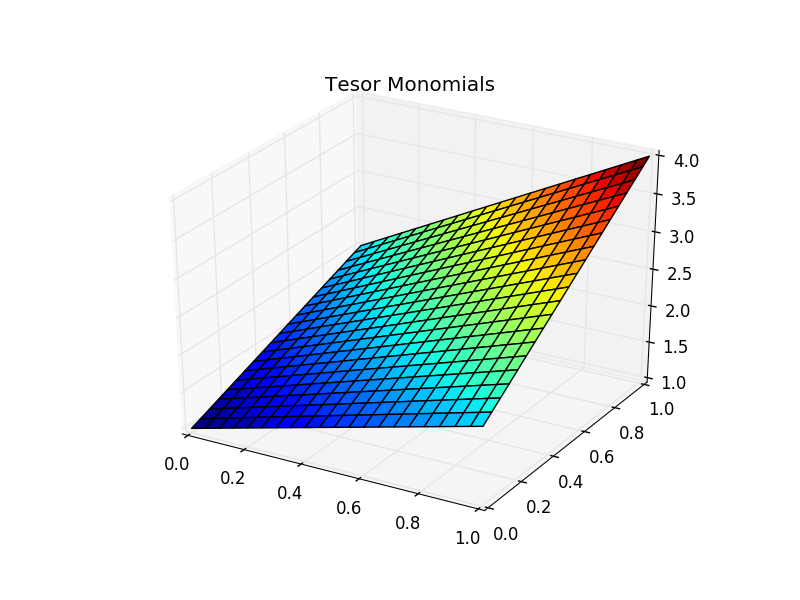
\includegraphics[width=0.7\linewidth]{anlmodels/tensor_monom}
  \caption{Tensor Monomials}
  \label{fig: tensor monomials}
\end{figure}

\begin{table}[H]
  \centering
  \begin{tabular}{c|c|c}
    Distribution & Mean & Variance \\\hline
    $\mathcal{U}[-1,1]$ & 1 & $\qty(\frac{4}{3})^N - 1$ \\
    $\mathcal{U}[0,1]$ & $\qty(\frac{3}{4})^N$ & $\qty(\frac{7}{3})^N - \qty(\frac{3}{4})^{2N}$ \\
    $\mathcal{N}[\mu,\sigma]$ & $\prod_{n=1}^N (\mu_{y_n}+1)$ & $\prod_{n=1}^N[(\mu_{y_n}+1)^2+\sigma_{y_n}^2]
    - \prod_{n=1}^N (\mu_{y_n}+1)^2$
  \end{tabular}
  \caption{Analytic Expressions for Tensor Monomial Case}
  \label{tab:tensormono moments}
\end{table}
For purposes of demonstration, we pick several increasing orders of dimensionality: three input variables, five variables, and
ten variables.

\subsection{Discussion}
As this polynomial contains only combinations of
first-order polynomials, we expect the Tensor Product index set construction method to be very efficient
in absolute error magnitude.  
As such, it will be difficult to observe the convergence rate for this method, as it converges exactly with 
first-order polynomials..
Because the model has infinite continuity, we expect all collocation-based
methods to be quite efficient.  Plots with the values and errors of the mean and standard deviation are given
for each of three (Figures \ref{fig:tensormono mean values 3} through \ref{fig:tensormono var errors 3}),
five (Figures \ref{fig:tensormono mean values 5} through \ref{fig:tensormono var errors 5}), 
and ten (Figures \ref{fig:tensormono mean values 10} through \ref{fig:tensormono var errors 10})
input parameters.  Note specially that TP exactly reproduces the original model with expansion order 1, so no convergence is
observed past the initial sampling point.

\subsection{3 Inputs}
The strength of collocation methods is clear for this small-dimensionality problem of three uncertain inputs.
The convergence on the
mean and standard deviation is swift for all the methods.  The convergence of the mean is instant for all methods, since
the linear nature of the problem means only the zeroth-order polynomial term is required to exactly reproduce the mean.
More convergence behavior can be seen for the standard deviation.
Because hyperbolic cross polynomials emphasize single-variable polynomials over cross terms, it is the slowest to reach
effectively zero error.  Similarly, the total degree quickly obtains most of the polynomials in the exact expansion,
but takes a few levels to include the term that has all the input variables in it.  Because first-order tensor product
polynomials is exactly the model itself, it converges instantly.
The adaptive SCgPC method initially explores high-order polynomials before finding the remaining tensor
monomials, which makes it less directly efficient than tensor product but otherwise desirable over the other
two static polynomial sets.
\begin{figure}[H]
  \centering
  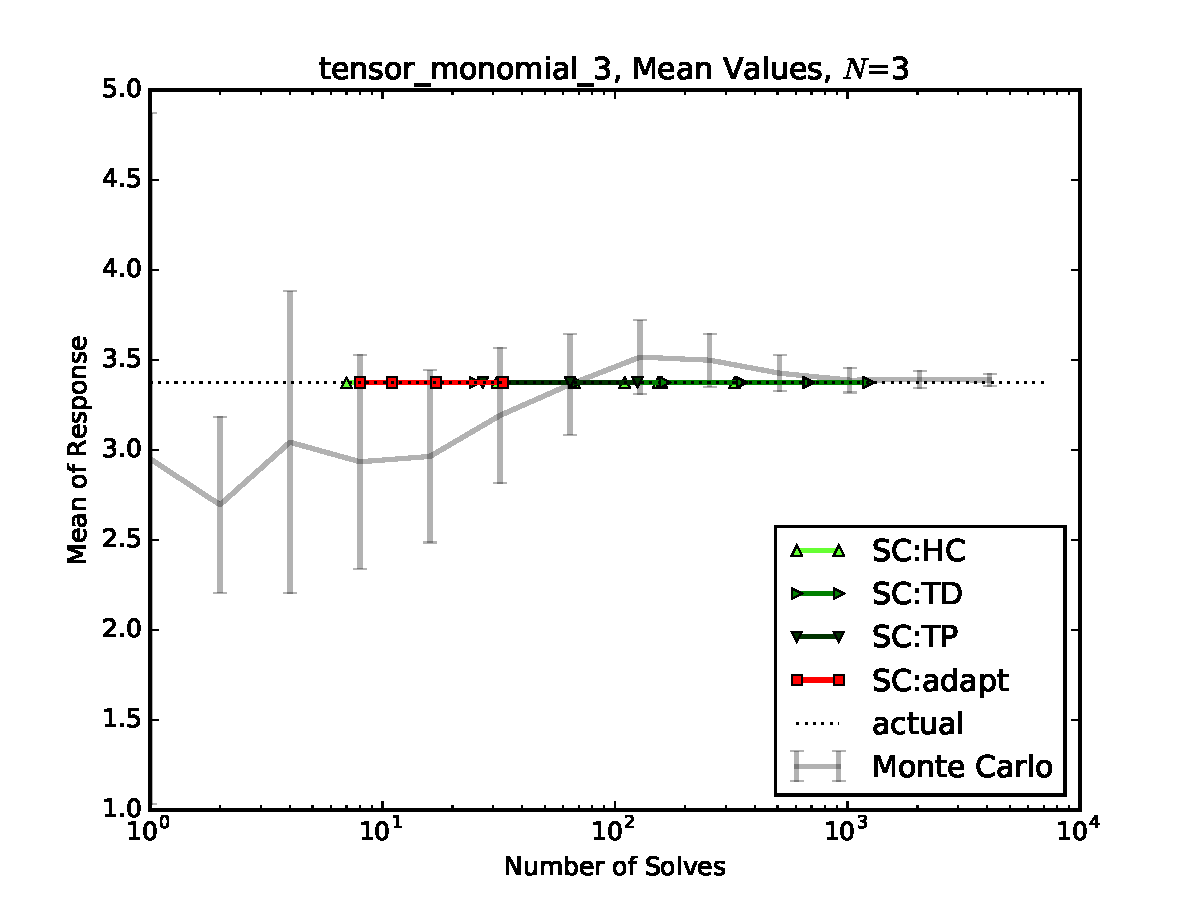
\includegraphics[width=0.7\linewidth]{anlmodels/tensor_monomial_3_mean_vals_nohdmr}
  \caption{Tensor Monomial, $N=3$, Mean Values}
  \label{fig:tensormono mean values 3}
\end{figure}
\begin{figure}[H]
  \centering
  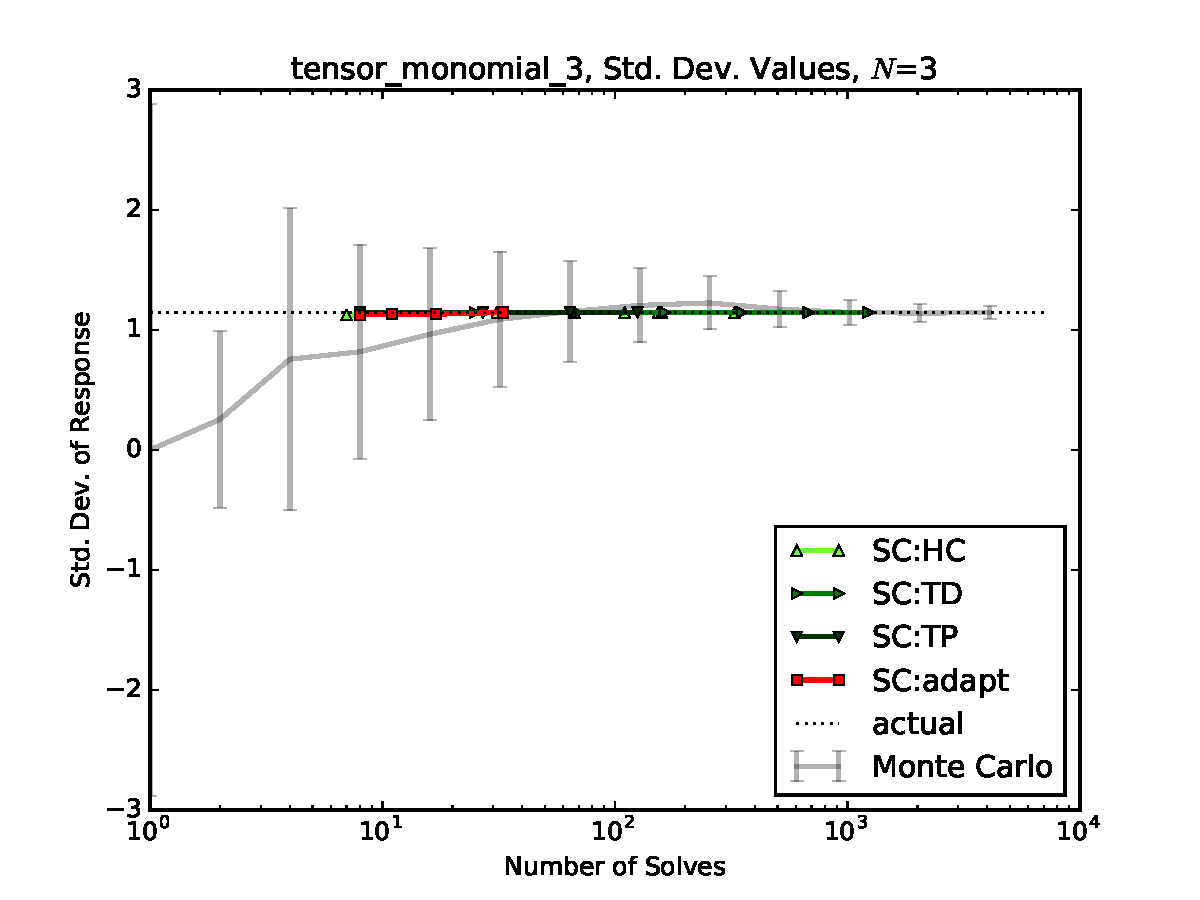
\includegraphics[width=0.7\linewidth]{anlmodels/tensor_monomial_3_var_vals_nohdmr}
  \caption{Tensor Monomial, $N=3$, Std. Dev. Values}
  \label{fig:tensormono var values 3}
\end{figure}

\begin{figure}[H]
  \centering
  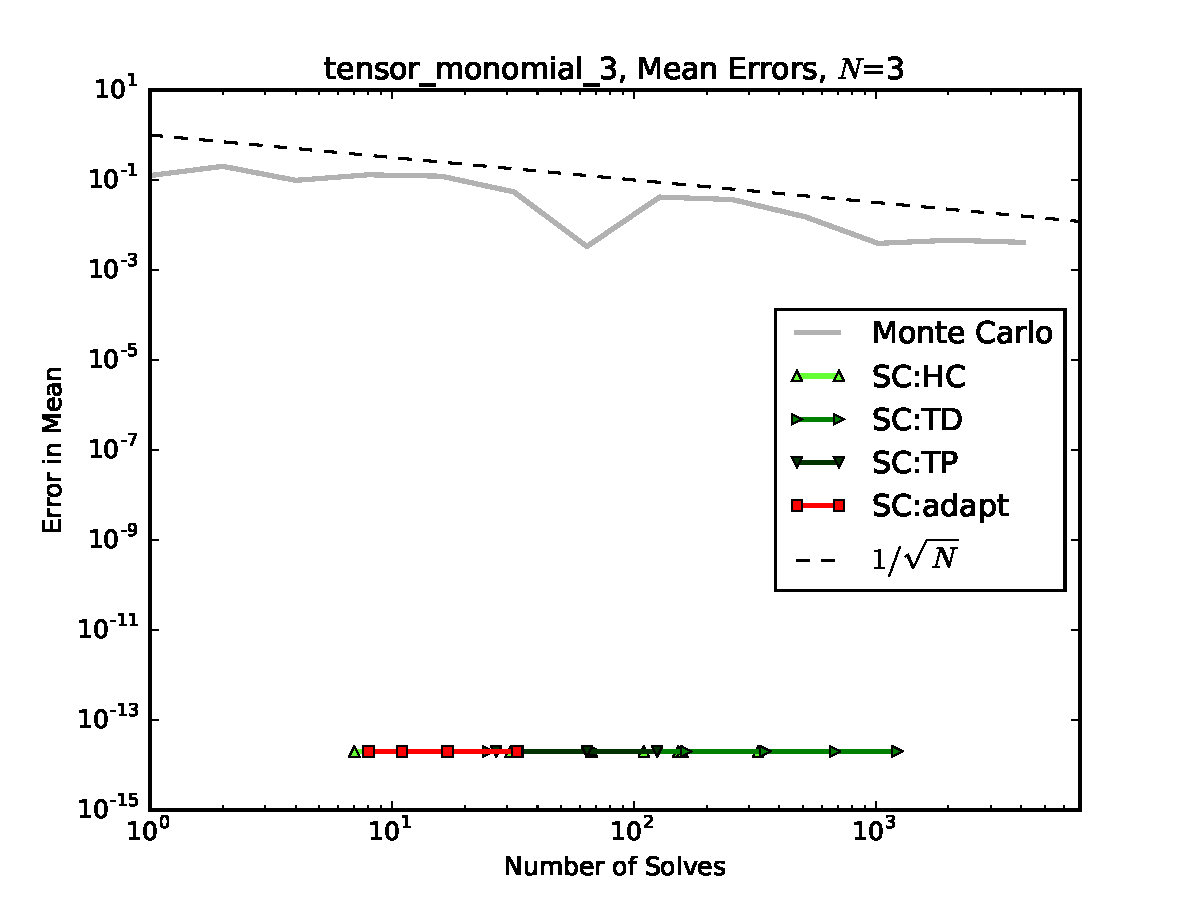
\includegraphics[width=0.7\linewidth]{anlmodels/tensor_monomial_3_mean_errs_nohdmr}
  \caption{Tensor Monomial, $N=3$, Mean Convergence}
  \label{fig:tensormono mean errors 3}
\end{figure}
\begin{figure}[H]
  \centering
  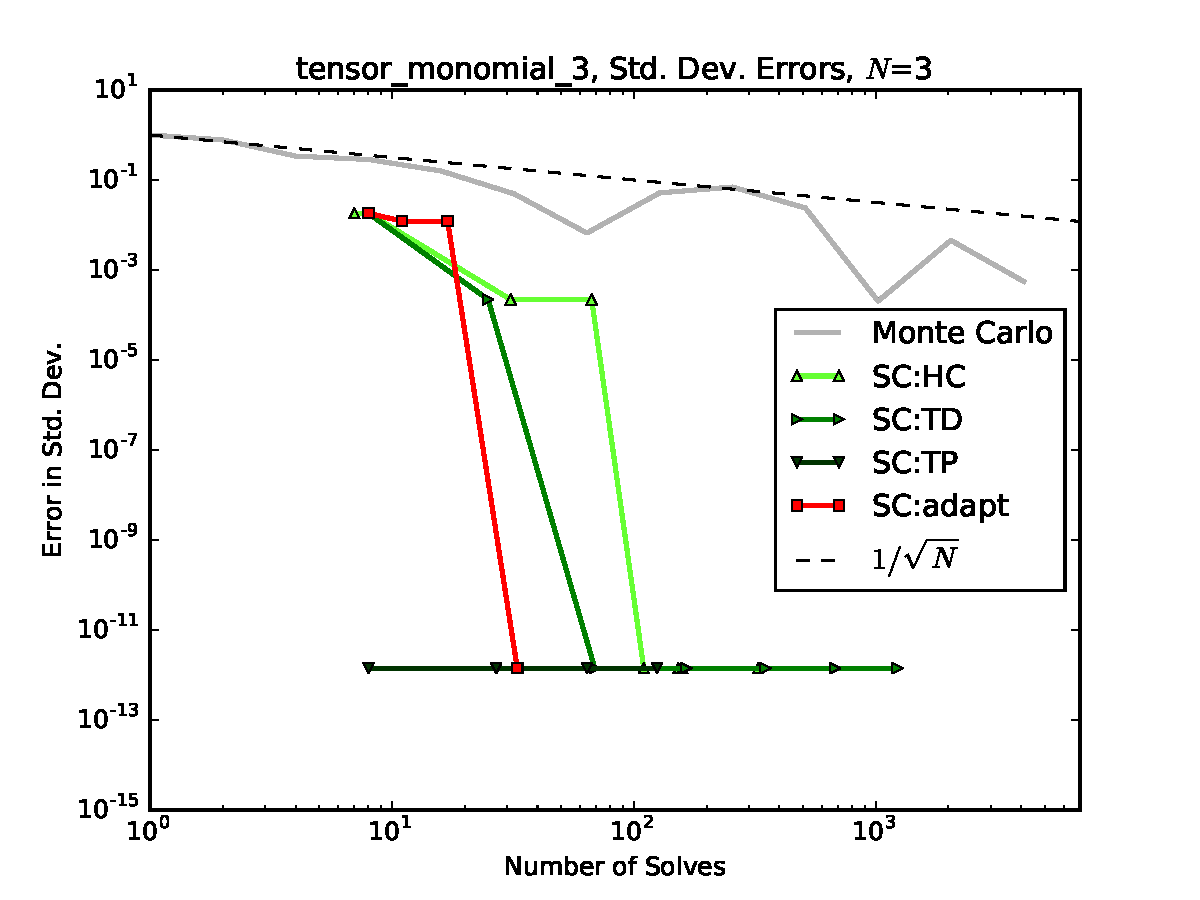
\includegraphics[width=0.7\linewidth]{anlmodels/tensor_monomial_3_variance_errs_nohdmr}
  \caption{Tensor Monomial, $N=3$, Std. Dev. Convergence}
  \label{fig:tensormono var errors 3}
\end{figure}

\subsection{5 Inputs}
While the convergence on the mean is still direct for the five-dimensional input problem, we begin to see
degradation in the convergence of collocation-based methods.  
As with the three variable case, the mean is trivial and obtained with the zeroth-order polynomial.  
Exponential
convergence can be seen for the total degree and hyperbolic cross polynomials, while the adaptive
method
is still exploring higher-order polynomials as more likely candidates for inclusion in the expansion and hasn't
seen the same rapid convergence curve yet.  This is a flaw in the default search parameters for the adaptive
algorithm when applied to this model.
Total Degree outperforms Hyperbolic Cross and Adaptive, as
the search algorithm struggles to find the optimal tensors of low-order polynomials required.  Hyperbolic
Cross is outperformed by Total Degree as expected for a problem with this level of regularity.
\begin{figure}[H]
  \centering
  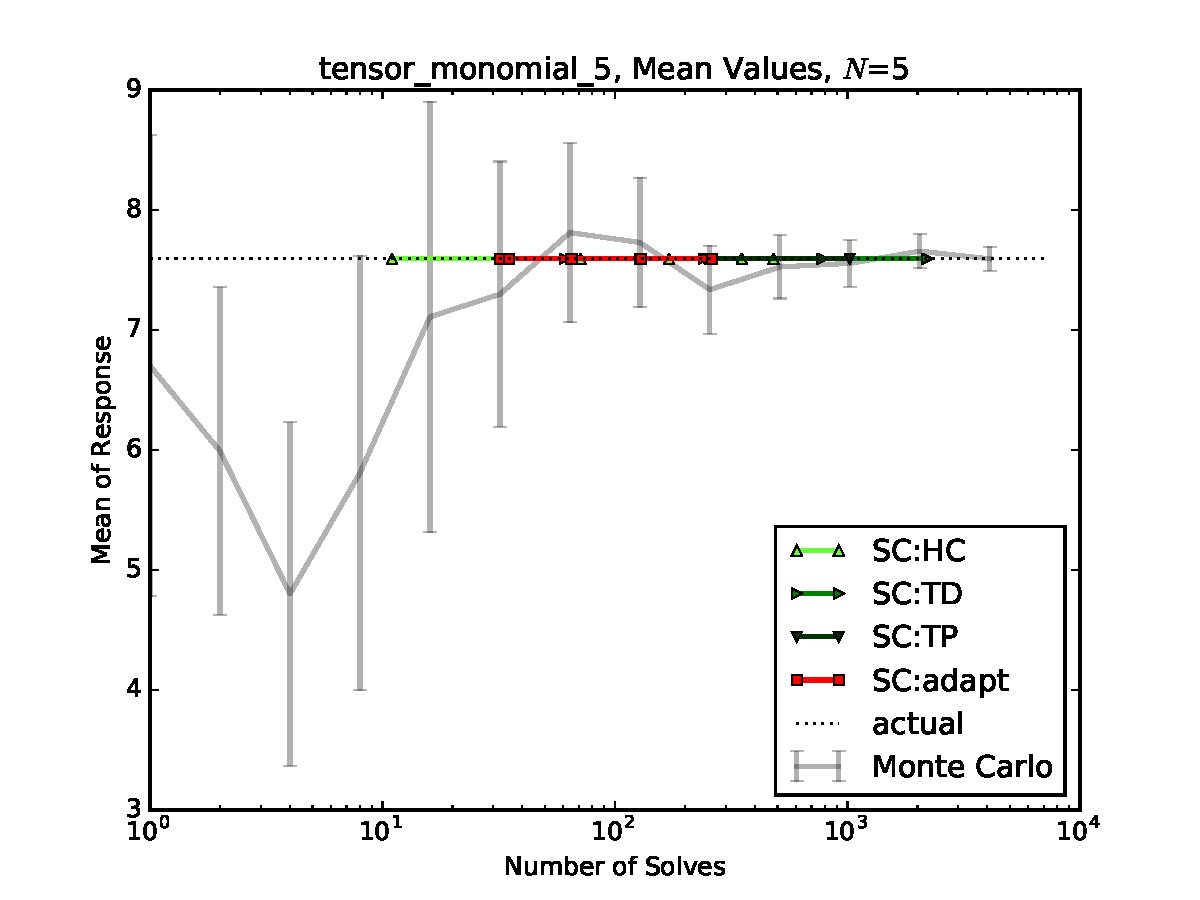
\includegraphics[width=0.7\linewidth]{anlmodels/tensor_monomial_5_mean_vals_nohdmr}
  \caption{Tensor Monomial, $N=5$, Mean Values}
  \label{fig:tensormono mean values 5}
\end{figure}
\begin{figure}[H]
  \centering
  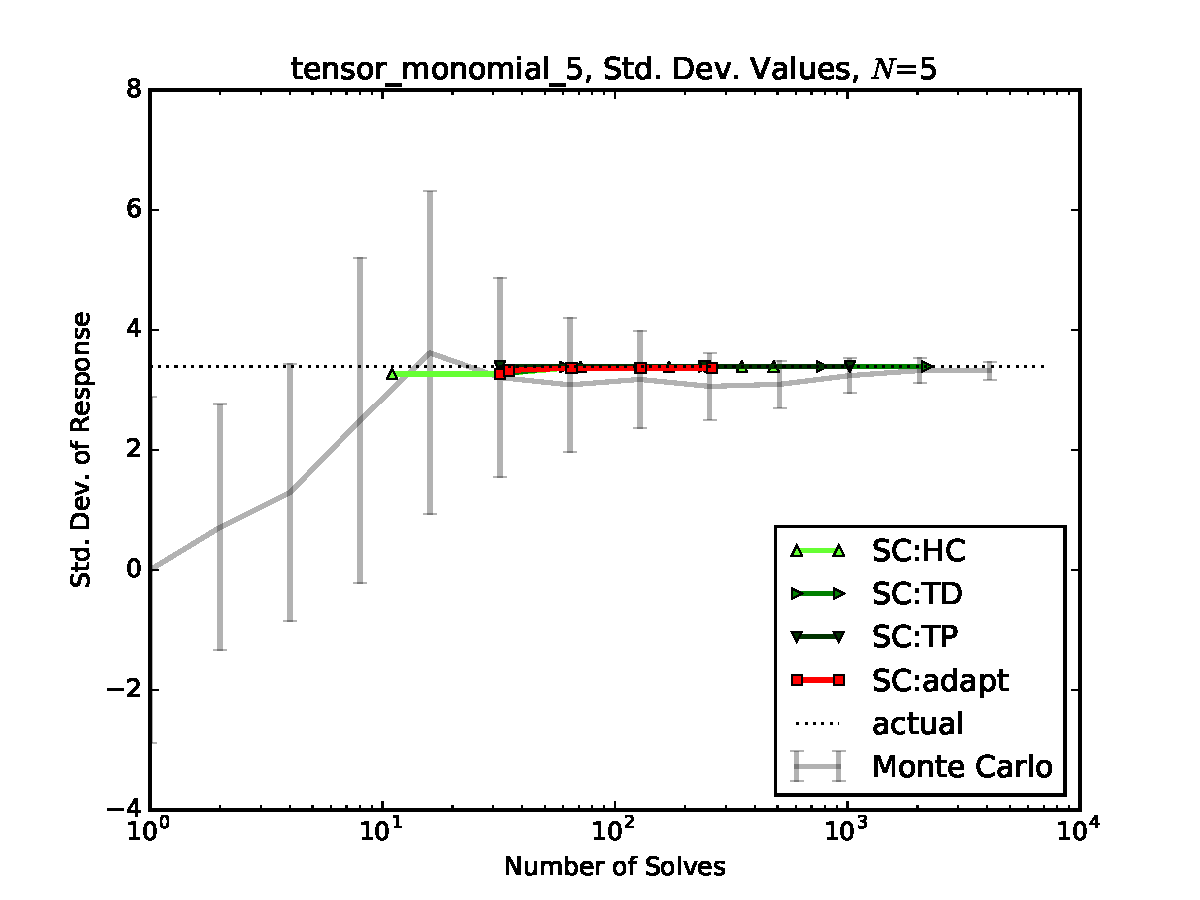
\includegraphics[width=0.7\linewidth]{anlmodels/tensor_monomial_5_var_vals_nohdmr}
  \caption{Tensor Monomial, $N=5$, Std. Dev. Values}
  \label{fig:tensormono var values 5}
\end{figure}

\begin{figure}[H]
  \centering
  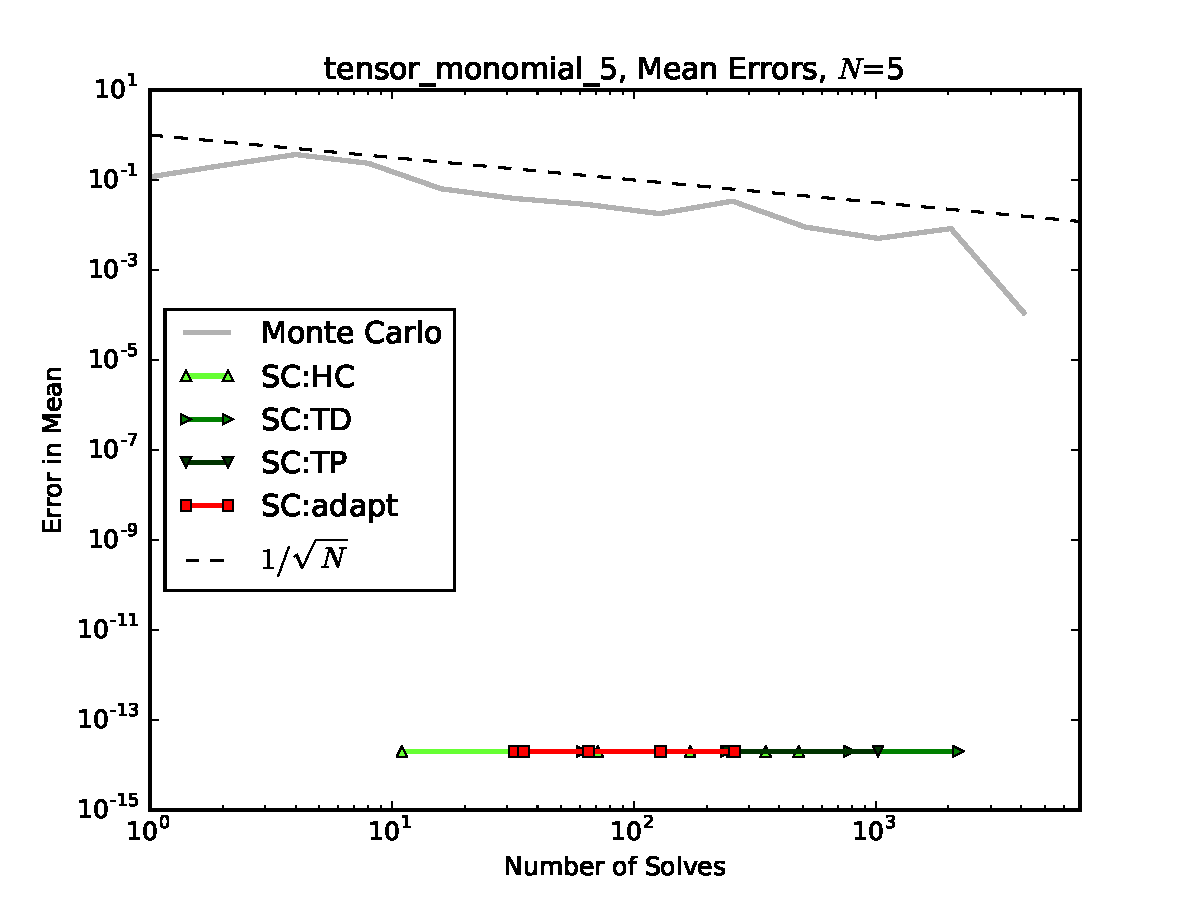
\includegraphics[width=0.7\linewidth]{anlmodels/tensor_monomial_5_mean_errs_nohdmr}
  \caption{Tensor Monomial, $N=5$, Mean Convergence}
  \label{fig:tensormono mean errors 5}
\end{figure}
\begin{figure}[H]
  \centering
  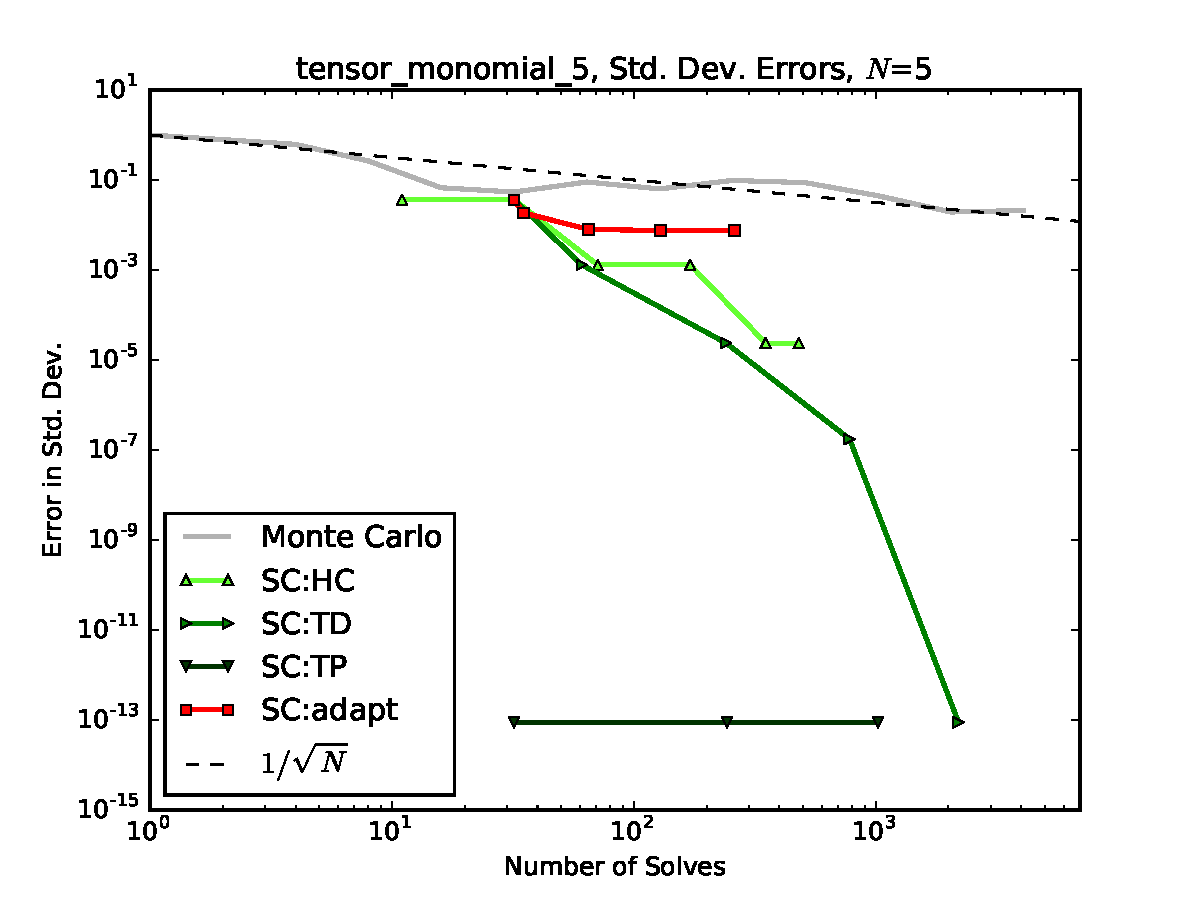
\includegraphics[width=0.7\linewidth]{anlmodels/tensor_monomial_5_variance_errs_nohdmr}
  \caption{Tensor Monomial, $N=5$, Std. Dev. Convergence}
  \label{fig:tensormono var errors 5}
\end{figure}

\subsection{10 Inputs}
As we increase to ten inputs, we see significant degradation of all the collocation methods in converging on
the standard deviation.  While it appears there might be exponential convergence, the curvature is quite large, and
only somewhat better than linear convergence is observed for up to 1000 computational solves.  One reason the
adaptive method does not perform more admirably for this case is the equal-weight importance of all the input
terms as well as the polynomial terms; the high-dimensional space takes considerable numbers of runs to
explore thoroughly, and this model contains some of the most difficult polynomials to find adaptively: those including
all of the inputs. 
\begin{figure}[H]
  \centering
  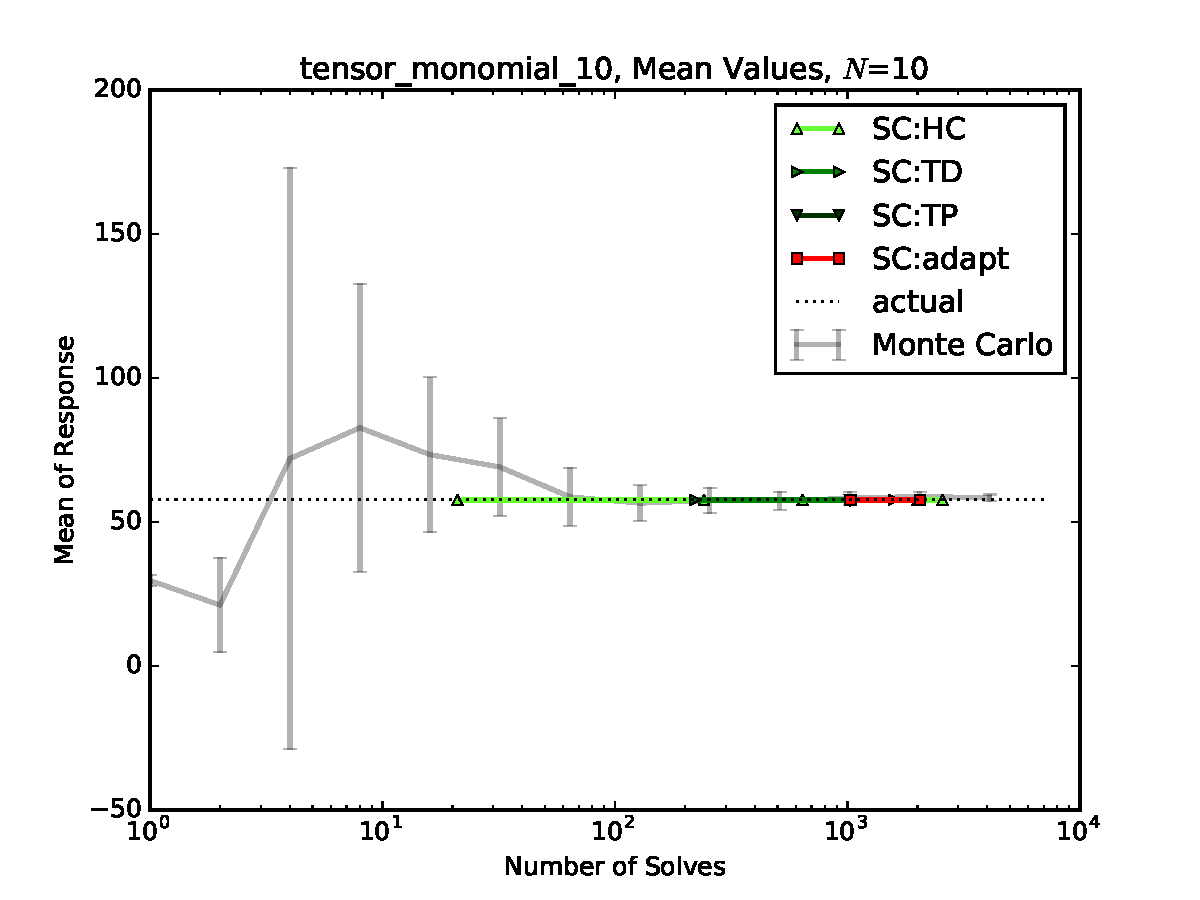
\includegraphics[width=0.7\linewidth]{anlmodels/tensor_monomial_10_mean_vals_nohdmr}
  \caption{Tensor Monomial, $N=10$, Mean Values}
  \label{fig:tensormono mean values 10}
\end{figure}
\begin{figure}[H]
  \centering
  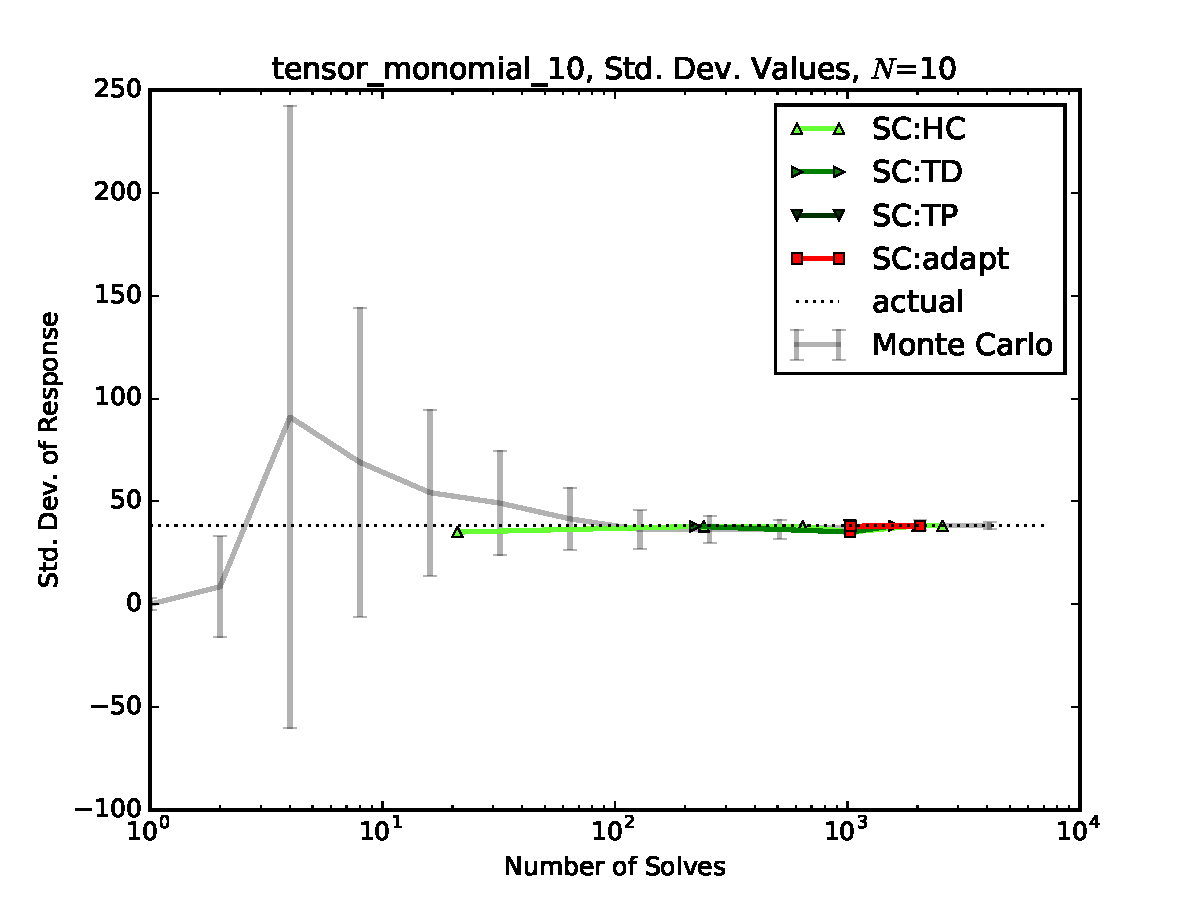
\includegraphics[width=0.7\linewidth]{anlmodels/tensor_monomial_10_var_vals_nohdmr}
  \caption{Tensor Monomial, $N=10$, Std. Dev. Values}
  \label{fig:tensormono var values 10}
\end{figure}

\begin{figure}[H]
  \centering
  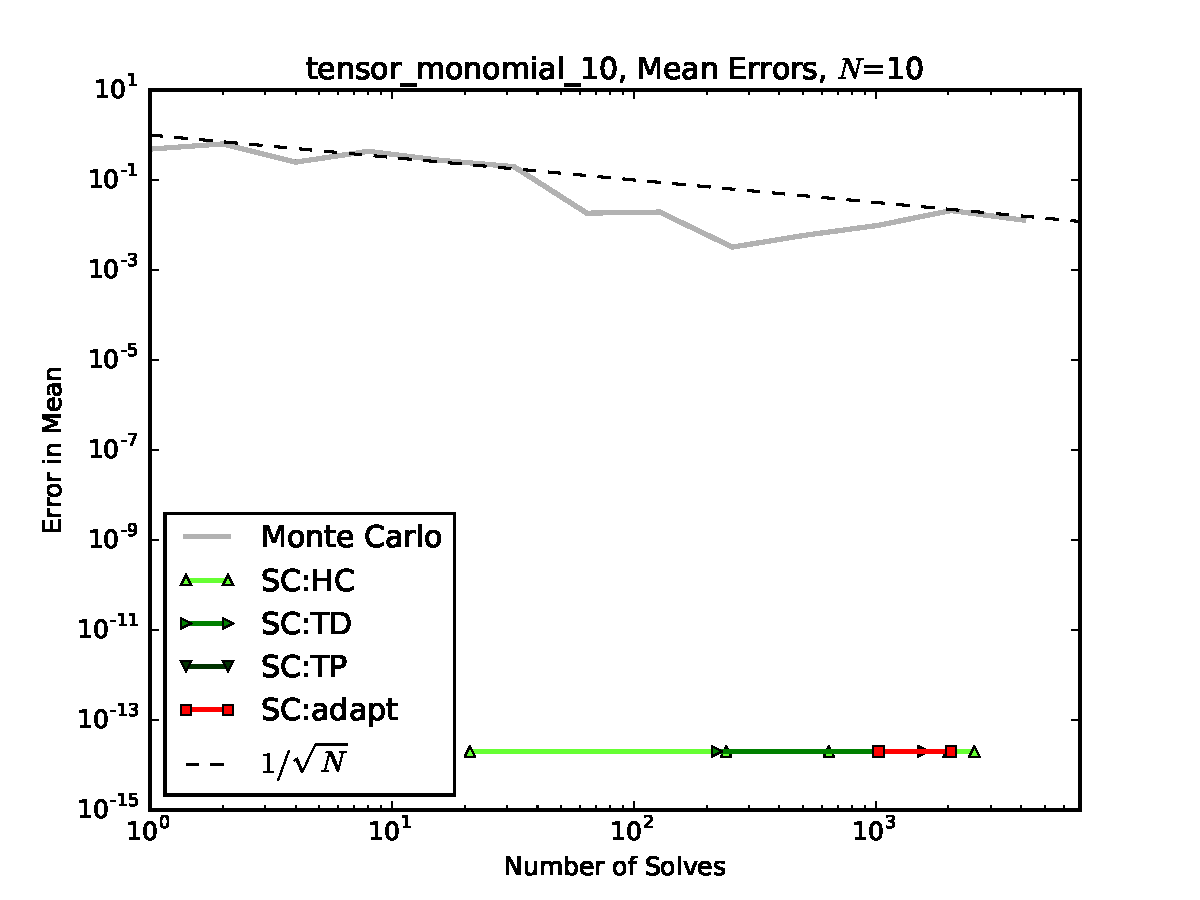
\includegraphics[width=0.7\linewidth]{anlmodels/tensor_monomial_10_mean_errs_nohdmr}
  \caption{Tensor Monomial, $N=10$, Mean Convergence}
  \label{fig:tensormono mean errors 10}
\end{figure}
\begin{figure}[H]
  \centering
  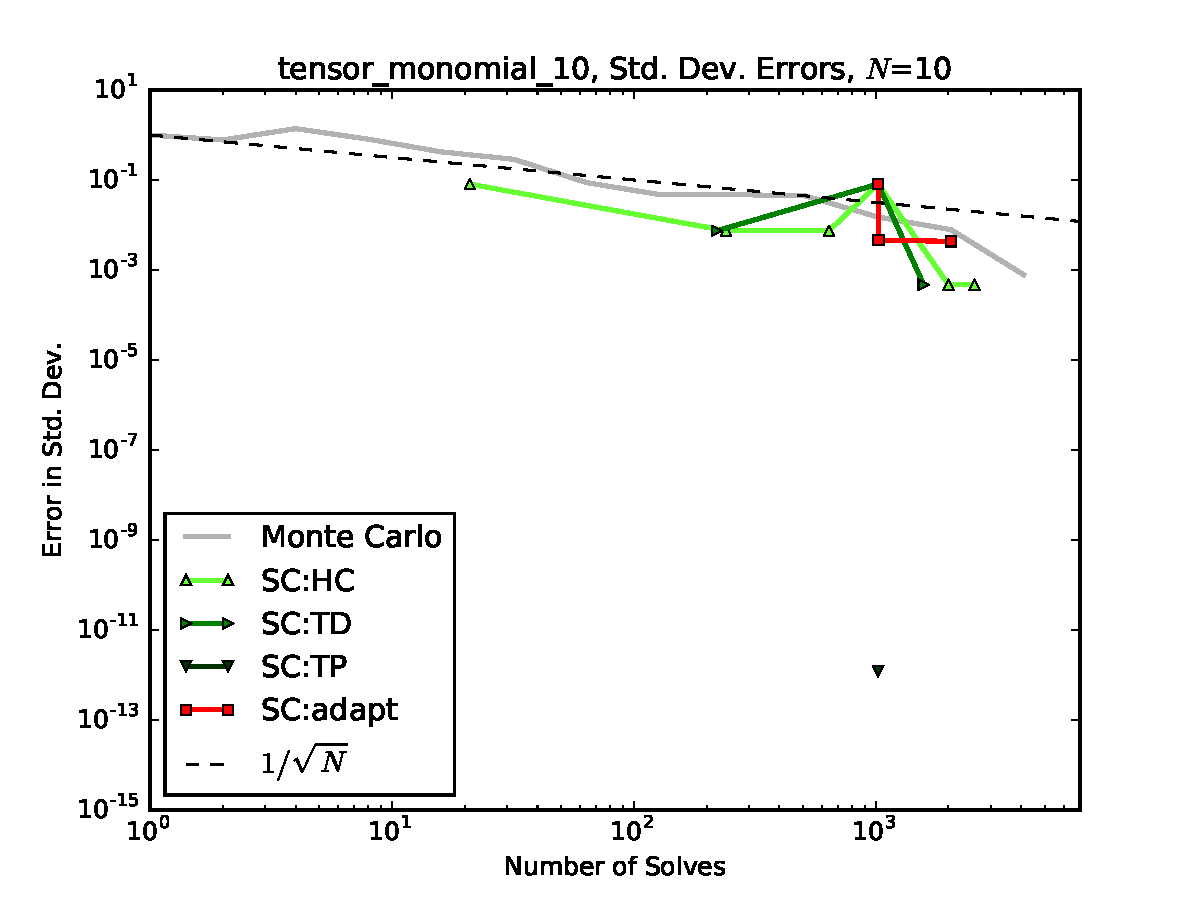
\includegraphics[width=0.7\linewidth]{anlmodels/tensor_monomial_10_variance_errs_nohdmr}
  \caption{Tensor Monomial, $N=10$, Std. Dev. Convergence}
  \label{fig:tensormono var errors 10}
\end{figure}


\section{Sudret Polynomial}
\subsection{Description}
The polynomial used by Sudret in his work \cite{sudret} is another tensor-like polynomial, and is a test case traditionally used to
identify convergence on sensitivity parameters.  It is similar to tensor monomials because it is constructed by the tensor
product of simple polynomials; in this case, Sudret used second-order polynomials.  As a result, only zeroth or second-order
polynomials exist in the expression.  Statistical moments are also quite straightforward for this model.
The mathematical expression for Sudret polynomials is
\begin{equation}
  u(Y) = \frac{1}{2^N}\prod_{n=1}^N (3y_n^2+1).
\end{equation}
The two-dimensional representation of this function is given in Figure \ref{fig: sudret}.
\begin{figure}[htb]
  \centering
  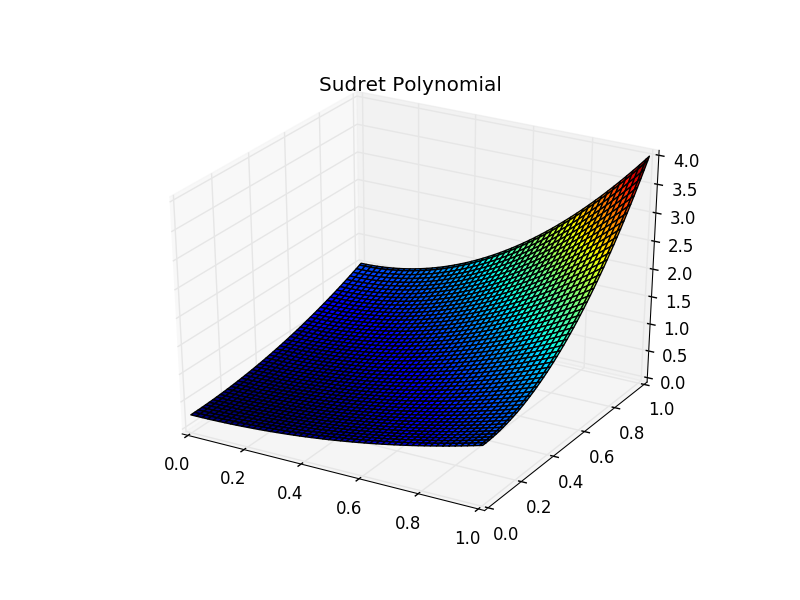
\includegraphics[width=0.7\linewidth]{anlmodels/sudret}
  \caption{Sudret Polynomial}
  \label{fig: sudret}
\end{figure}
The variables are distributed uniformly on [0,1].

The statistical moments and sensitivities are given in
Table \ref{tab:sudret}, where $\mathcal{S}_n$ is the global Sobol sensitivity of $u(Y)$ to perturbations in
$y_n$.

\begin{table}[H]
  \centering
  \begin{tabular}{c c}
    Statistic & Expression \\\hline
    Mean & 1 \\
    Variance & $\qty(\frac{6}{5})^N - 1$ \\
    $\mathcal{S}_n$ & $\frac{5^{-n}}{(6/5)^N-1}$
  \end{tabular}
  \caption{Analytic Expressions for Sudret Case}
  \label{tab:sudret}
\end{table}
Because of its similarity to tensor polynomials, the cases we show are three inputs and five inputs.

\subsection{Discussion}
The Sudret polynomial model is a near neighbor to the
tensor monomials model; however, it includes only even-ordered polynomials, which provides more of a challenge
to the adaptive method.  Because the model is still a tensor product, the tensor product collocation method 
converges most directly in all dimensionality cases.  An interesting feature of the standard deviation for
this model is that the first-order expansions tend to estimate the variance more accurately than the
second-order expansions; as a result, it appears that the error is very small then grows rapidly.  This is
misleading to considering convergence, however, as the initial approximation is exhibits some cancellation of
errors to obtains such an ``accurate'' result.

\subsection{3 Inputs}
As with the tensor monomials, we see a good rate of convergence for many of the polynomial methods.  With
this model, the mean is not trivially given by the zeroth-order polynomial, and so some convergence is seen
in obtaining the expected value.  The total degree and adaptive methods converge at a similar rate for
the mean, while the hyperbolic cross demonstrates its poor convergence for highly regular systems with
nonlinear cross-term effects.  Quickest to converge (aside from the tensor product case) is the adaptive
SCgPC, because its search method allows it to discover the second-order polynomials quickly.

Similar behavior is seen for the standard deviation.
The tensor product still converges very rapidly, and total degree shows a good rate of convergence, while
hyperbolic cross demonstrates poor convergence.
\begin{figure}[H]
  \centering
  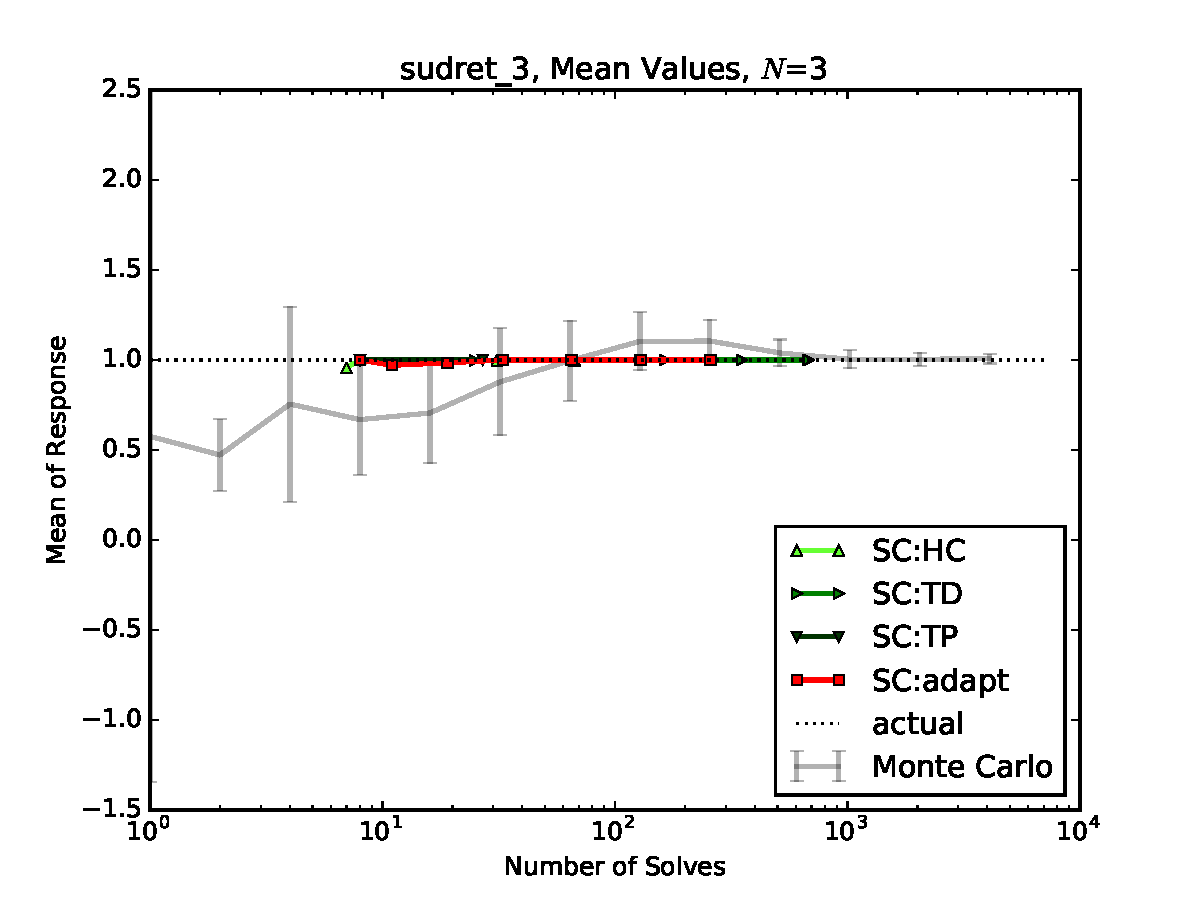
\includegraphics[width=0.7\linewidth]{anlmodels/sudret_3_mean_vals_nohdmr}
  \caption{Sudret Polynomial, $N=3$, Mean Values}
  \label{fig:sudretpoly mean values 3}
\end{figure}
\begin{figure}[H]
  \centering
  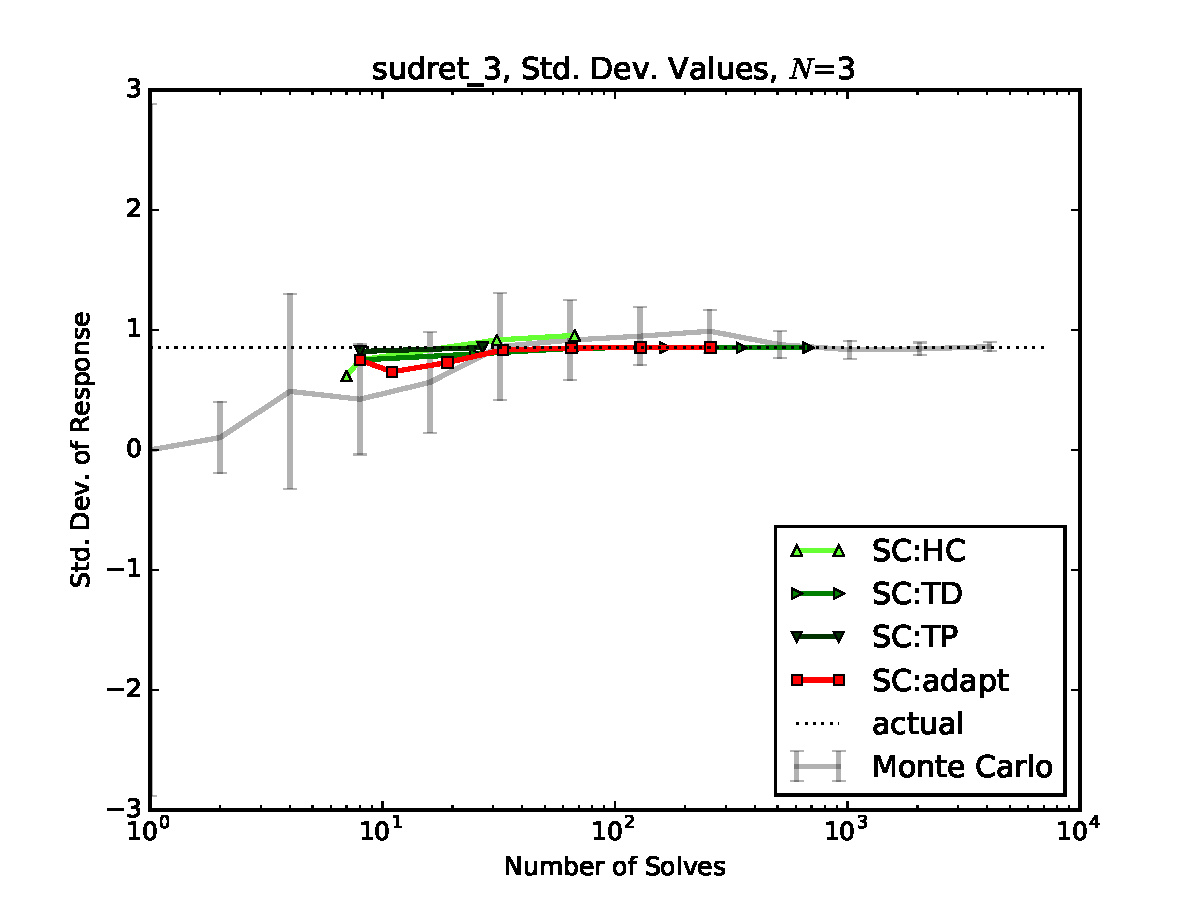
\includegraphics[width=0.7\linewidth]{anlmodels/sudret_3_var_vals_nohdmr}
  \caption{Sudret Polynomial, $N=3$, Std. Dev. Values}
  \label{fig:sudretpoly var values 3}
\end{figure}

\begin{figure}[H]
  \centering
  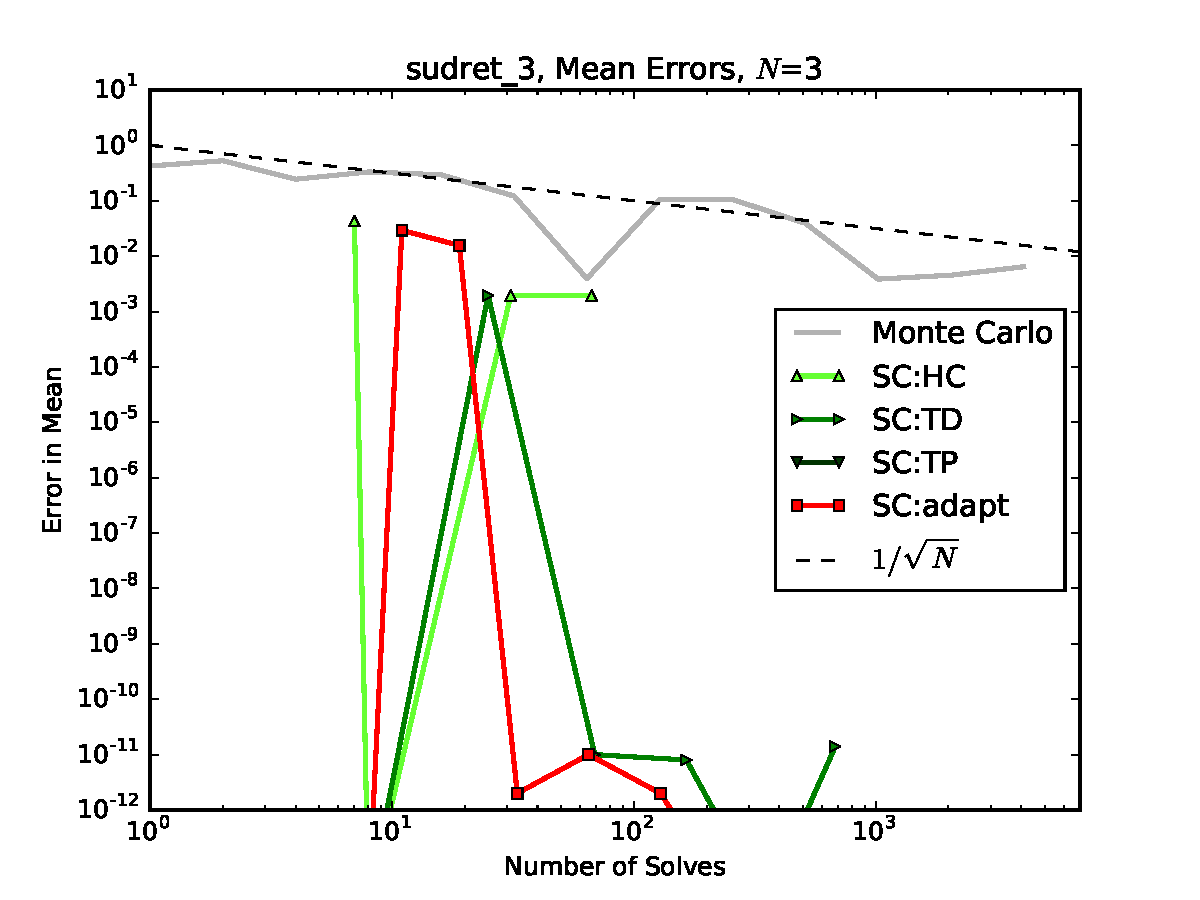
\includegraphics[width=0.7\linewidth]{anlmodels/sudret_3_mean_errs_nohdmr}
  \caption{Sudret Polynomial, $N=3$, Mean Convergence}
  \label{fig:sudretpoly mean errors 3}
\end{figure}
\begin{figure}[H]
  \centering
  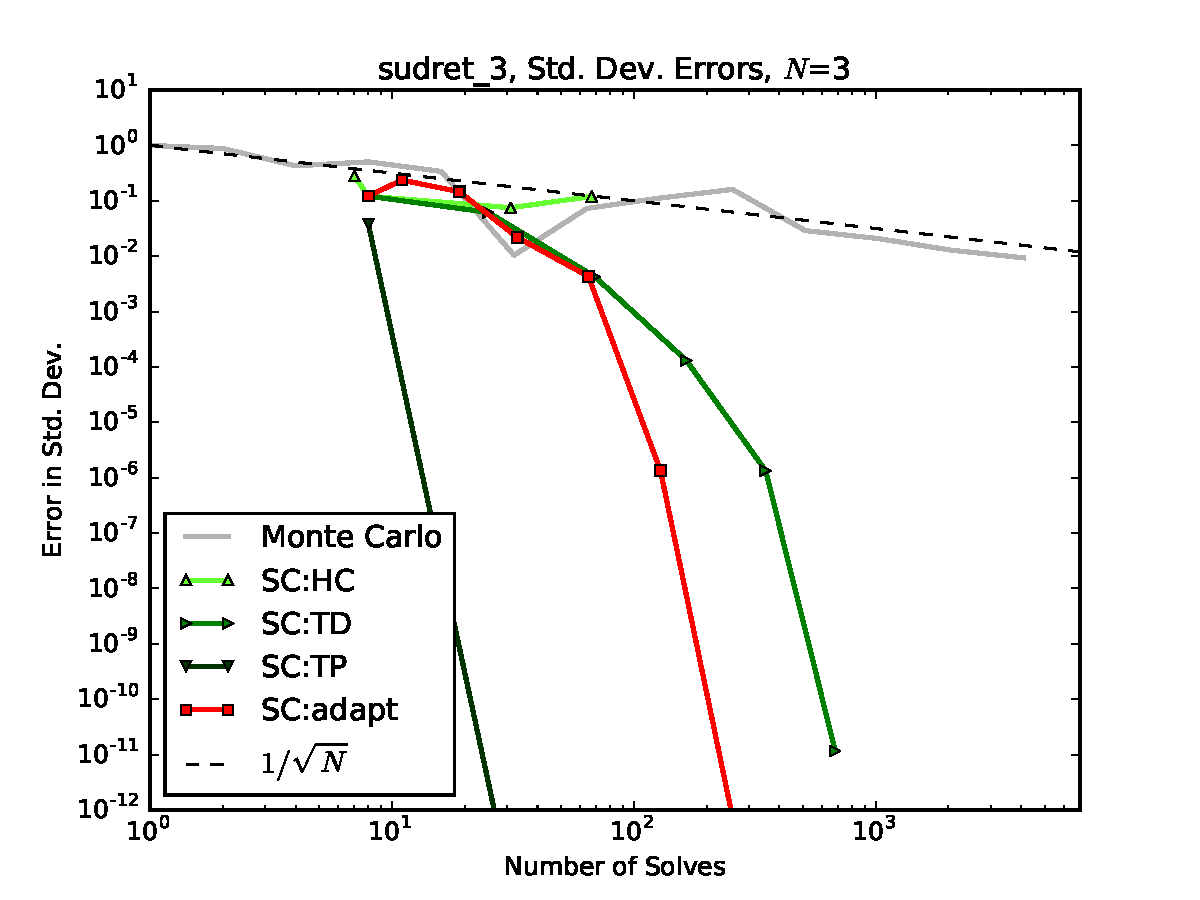
\includegraphics[width=0.7\linewidth]{anlmodels/sudret_3_variance_errs_nohdmr}
  \caption{Sudret Polynomial, $N=3$, Std. Dev. Convergence}
  \label{fig:sudretpoly var errors 3}
\end{figure}

\subsection{5 Inputs}
In the five-input case for the Sudret polynomials, we see slower but strong convergence for adaptive and
total degree methods.
For the mean, each method is showing some level of exponential convergence, with the exception of the
hyperbolic cross method.  For the standard deviation,
however, the radius of curvature for the convergence is quite large.  This demonstrates the negative impact
growing input spaces have on the effectiveness of collocation methods in comparison with Monte Carlo.
\begin{figure}[H]
  \centering
  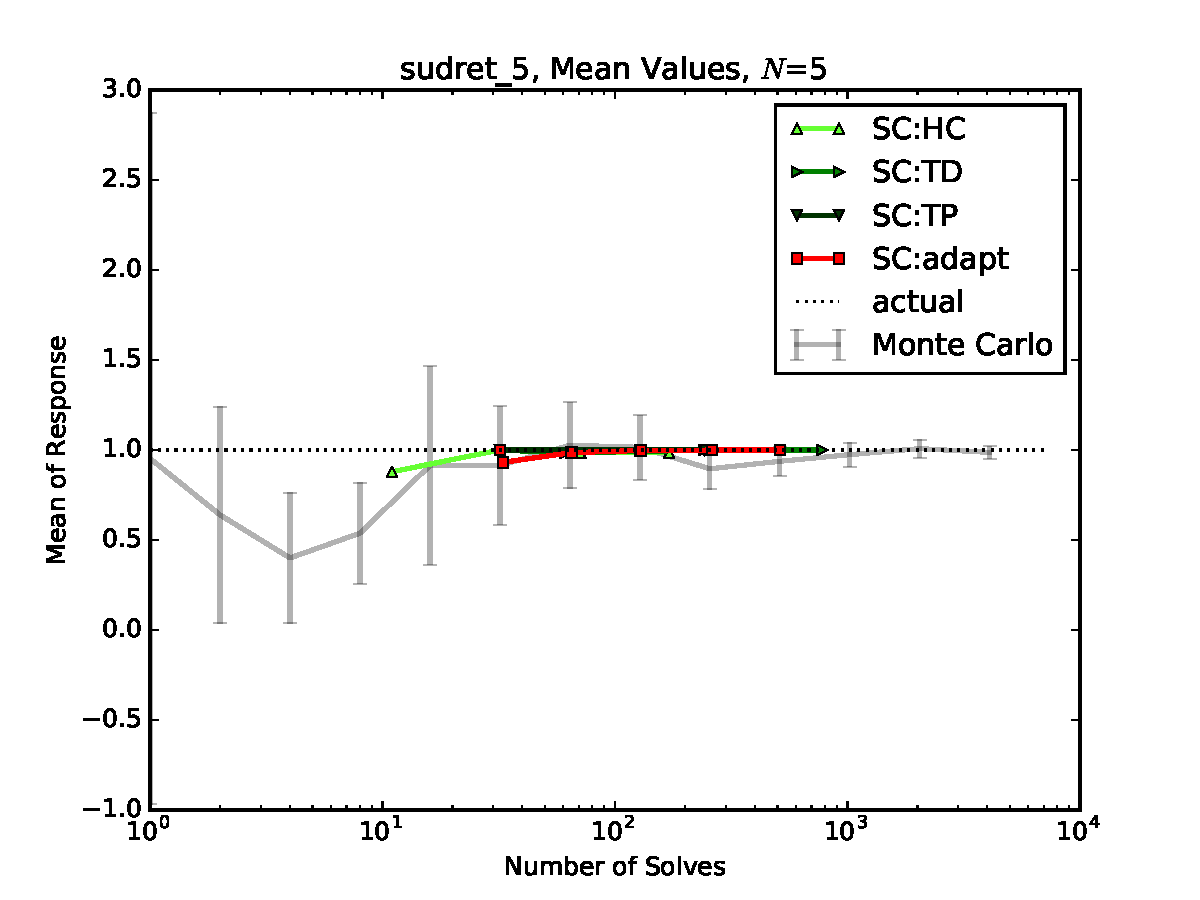
\includegraphics[width=0.7\linewidth]{anlmodels/sudret_5_mean_vals_nohdmr}
  \caption{Sudret Polynomial, $N=5$, Mean Values}
  \label{fig:sudretpoly mean values 5}
\end{figure}
\begin{figure}[H]
  \centering
  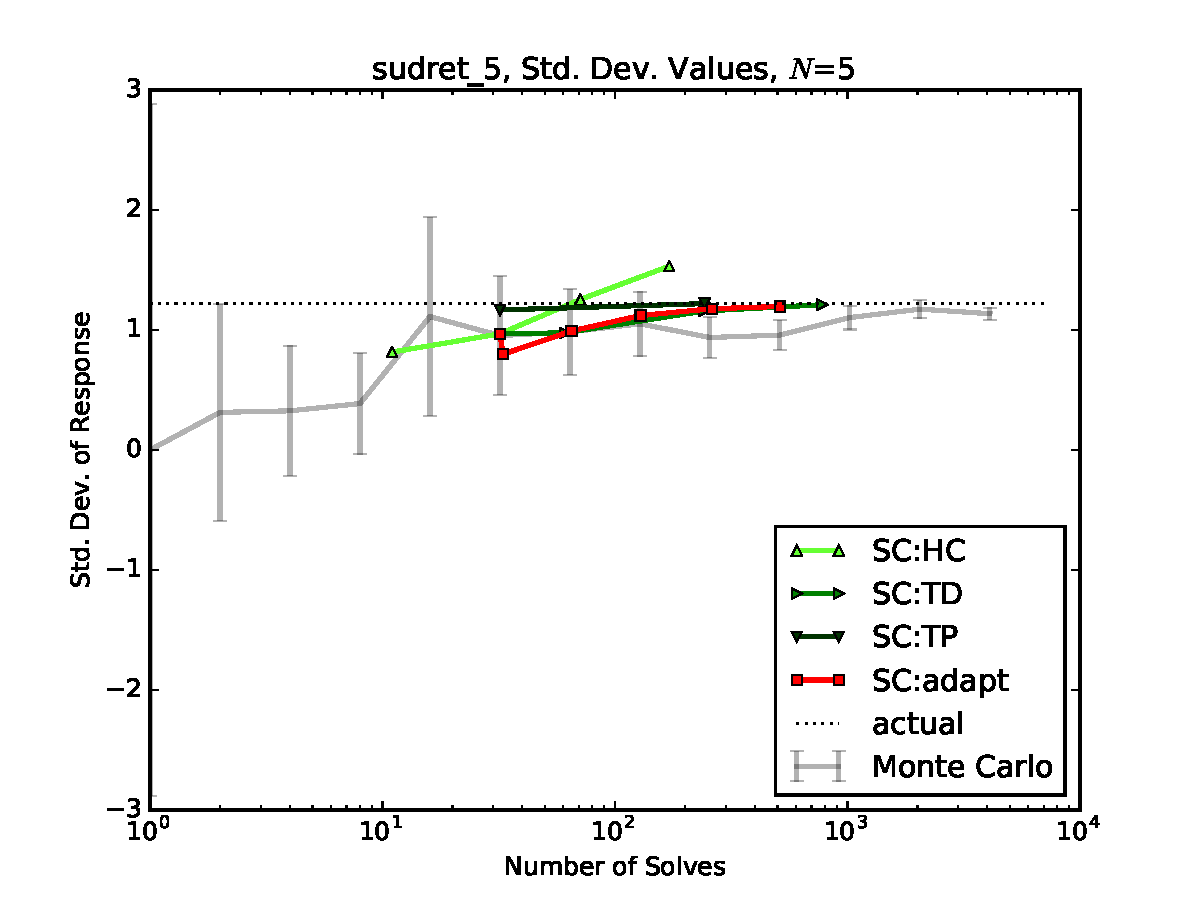
\includegraphics[width=0.7\linewidth]{anlmodels/sudret_5_var_vals_nohdmr}
  \caption{Sudret Polynomial, $N=5$, Std. Dev. Values}
  \label{fig:sudretpoly var values 5}
\end{figure}

\begin{figure}[H]
  \centering
  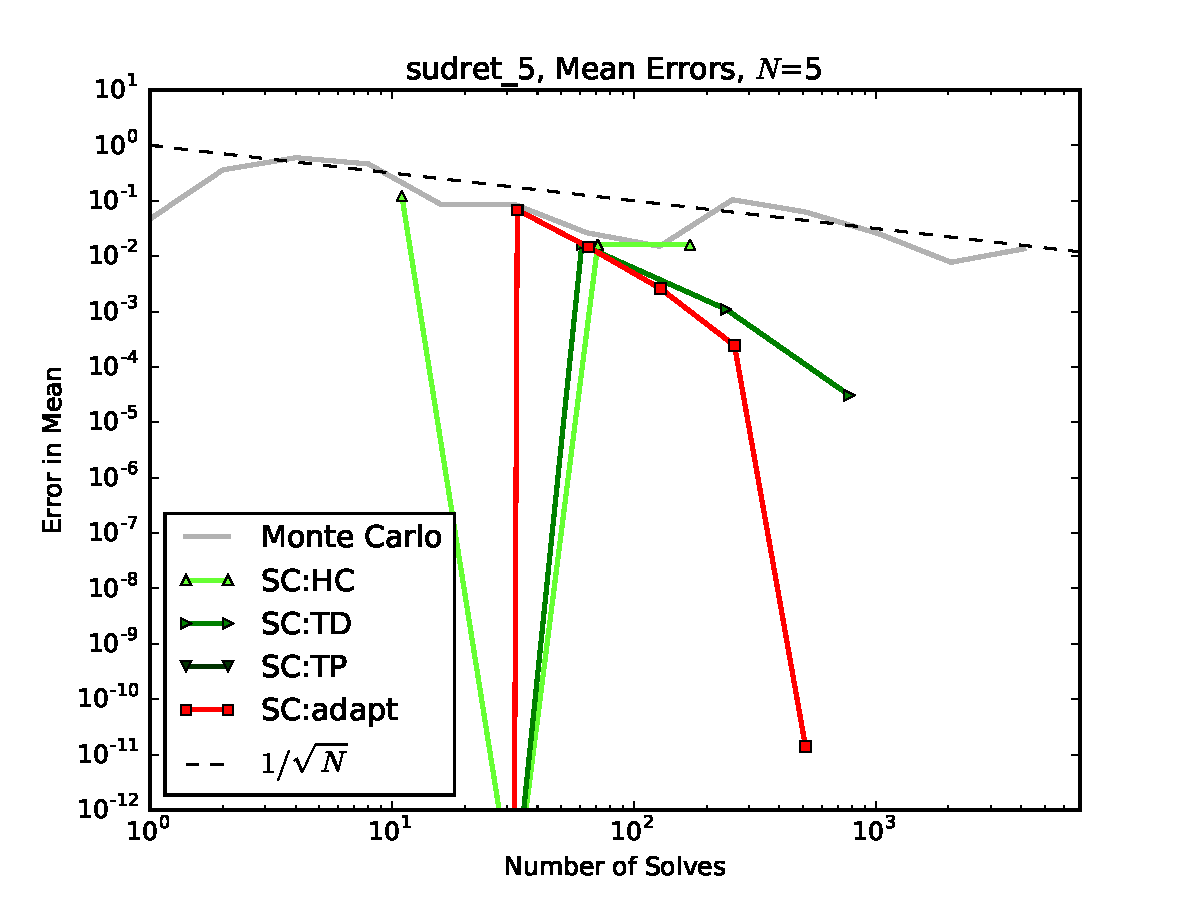
\includegraphics[width=0.7\linewidth]{anlmodels/sudret_5_mean_errs_nohdmr}
  \caption{Sudret Polynomial, $N=5$, Mean Convergence}
  \label{fig:sudretpoly mean errors 5}
\end{figure}
\begin{figure}[H]
  \centering
  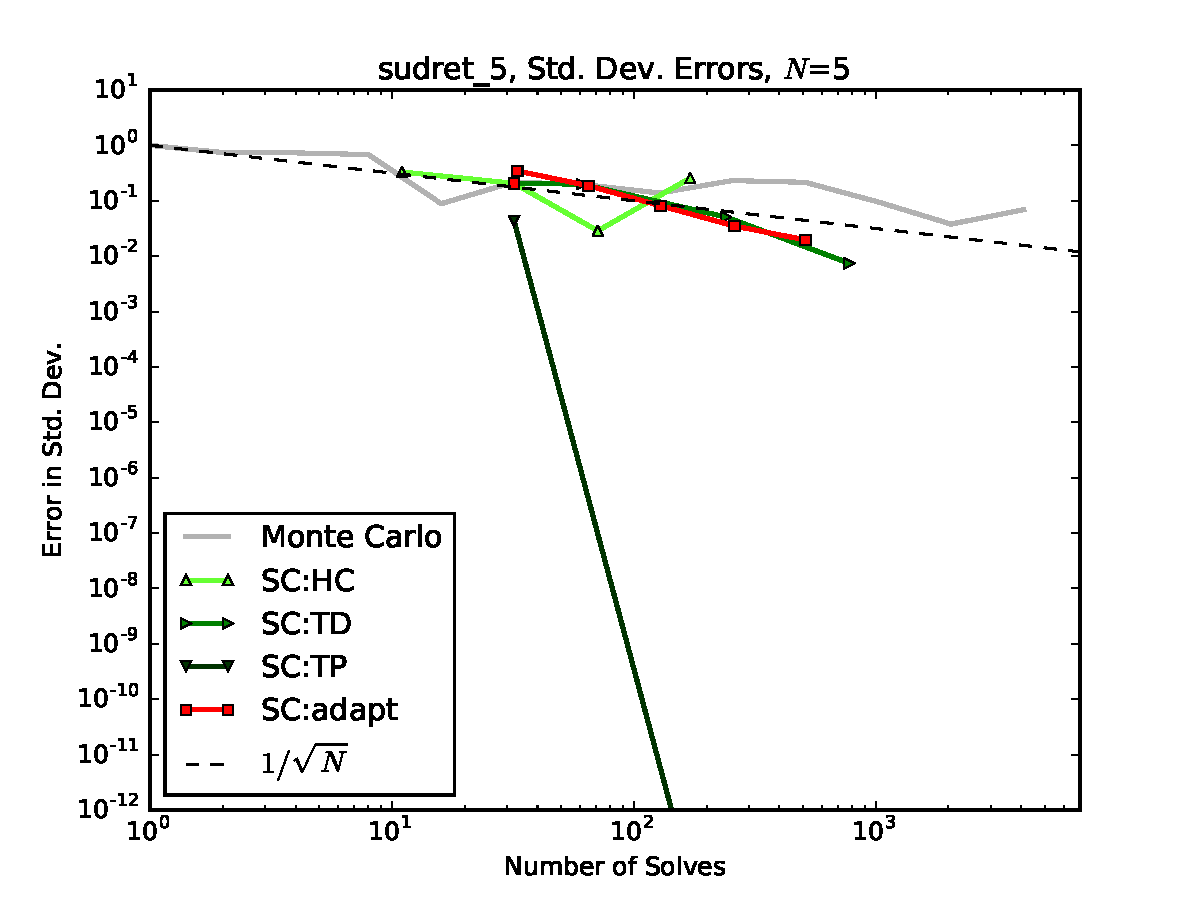
\includegraphics[width=0.7\linewidth]{anlmodels/sudret_5_variance_errs_nohdmr}
  \caption{Sudret Polynomial, $N=5$, Std. Dev. Convergence}
  \label{fig:sudretpoly var errors 5}
\end{figure}


\section{Attenuation}
\subsection{Description}
While this model is a tensor product and analytic, it also is the solution to a physical problem.
Consider a one-dimensional geometry that consists of a material with unit length and vacuum to the left and
right of the material.  We consider a beam of neutral particles that have a probability of interacting
with the material through absorption, or passing through it.  This beam enters the material on the left
and exits on the right with a fraction of its original flux.
The quantity of interest is the percent of particles that pass through the material without interacting
anywhere along its length.  The boundary conditions for this problem are a constant positive current on the 
left boundary, and a vacuum boundary on the right boundary.

This model represents an idealized single-dimension system where an beam of particles impinges on a
purely-absorbing material with total scaled length of 1.
The material is divided into $N$ segments, each of which
has a distinct uncertain interaction cross section $y_n$.  The cross section has units of probable interactions
per unit length, and the integral of a cross section over a length provides the probability of interaction
within that length.  The solution takes the form
\begin{equation}
  u(Y) = \prod_{n=1}^N \exp(-y_n/N).
\end{equation}
The two-dimensional representation of this function is given in Figure \ref{fig: attenuation}.
\begin{figure}[htb]
  \centering
  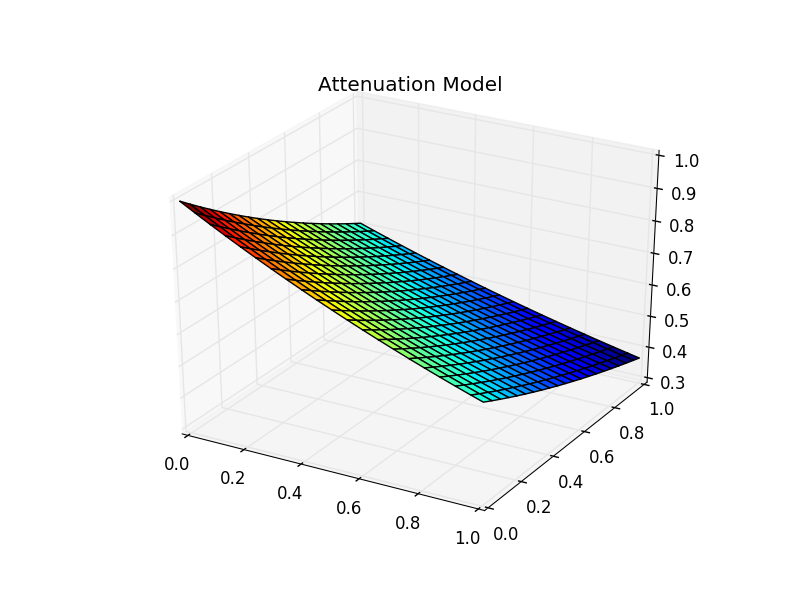
\includegraphics[width=0.7\linewidth]{anlmodels/attenuate}
  \caption{Attenuation Model}
  \label{fig: attenuation}
\end{figure}
Because negative cross sections have dubious physical meaning, we restrict the distribution cases to uniform
on [0,1] as well as normally-distributed on [$\mu,\sigma$].  A summary of analytic statistics is given in
Table \ref{tab:attenuation moments}.

\begin{table}[H]
  \centering
  \begin{tabular}{c|c|c}
    Distribution & Mean & Variance \\\hline
    $\mathcal{U}[0,1]$ & $\qty[N\qty(1-e^{-1/N})]^N$ & $\qty[\frac{N}{2}\qty(1-e^{-2/N})]^N -
                       \qty[N\qty(1-e^{-1/N})]^{2N}$ \\
    $\mathcal{N}[\mu,\sigma]$ & $\prod_{n=1}^N \exp\qty[\frac{\sigma_{y_n}^2}{2N^2}-\frac{\mu_{y_n}}{N}]$
    & $\prod_{n=1}^N \exp\qty[\frac{2\sigma_{y_n}^2}{N^2} - \frac{2\mu_{y_n}}{N}]$
  \end{tabular}
  \caption{Analytic Expressions for Attenuation Case}
  \label{tab:attenuation moments}
\end{table}

This model has some interesting properties to demonstrate performance of polynomial-based UQ methods.  First,
because the solution is a product of exponential functions, it cannot be exactly represented by a finite
number of polynomials.  Second, the Taylor development of the exponential function (about the origin) 
includes all increasing polynomial orders,
\begin{equation}
e^{ay} = 1 - ay + \frac{(ay)^2}{2} - \frac{(ay)^3}{6} + \frac{(ay)^4}{24} - \frac{(ay)^5}{120} + \mathcal{O}(y^6).
\end{equation}
As a result, the product of several exponential functions is effectively a tensor combination of
polynomials for each dimension.  The coefficients of higher-order polynomials are smaller than lower-order
polynomials; further, coefficients for combined polynomials have larger coefficients than single-dimensional
polynomials with the same effective order.  For example, for a two-dimensional exponential function and
considering effective fourth-order polynomials, the coefficient for $y_1^2y_2^2$ is $a_1^2a_2^2/4$, while the
coefficient for $y_1^4$ is $a^4/24$.

\subsection{Discussion}
Similar to the tensor monomial model and Sudret
polynomial model, the attenuation model can be expanded as the infinite sum of ever-increasing polynomials,
making it tensor product in shape.  However, unlike the previous two models, the magnitude of the contribution
from the higher-order polynomials decreases swiftly, making lower-order polynomials more characteristic of the
model in general.  Because this model is still a tensor model and the response is infinitely continuous,
we expect to see a similar trend in the most effective methods for polynomial expansion.

\subsection{2 Inputs}
With only two input parameters, we see excellent convergence for all methods for the mean, while Hyperbolic
Cross struggles to accurately represent the standard deviation.  As mentioned in the description, this is
likely because monomials are less important in the Taylor representation, while Hyperbolic Cross emphasizes
monomials over cross terms.  Interestingly, while Tensor
Product demonstrates the smallest error, its apparent curvature is slightly larger than for the other methods.
Because of the small input space, the total degree, hyperbolic cross, and adaptive methods all perform
similarly.  Because the adaptive method uses the impact of previous polynomials to choose future polynomials,
its convergence rate appears to improve as it continues.
\begin{figure}[H]
  \centering
  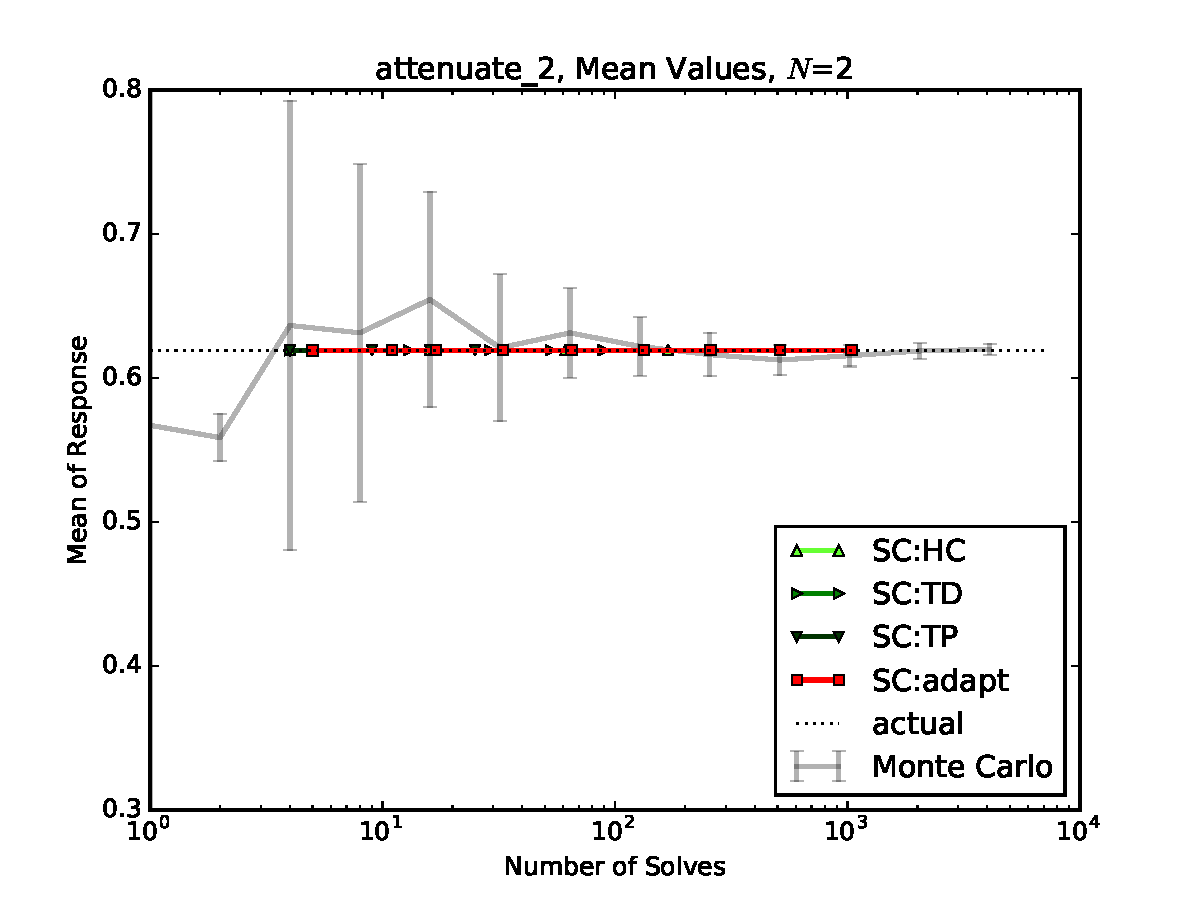
\includegraphics[width=0.7\linewidth]{anlmodels/attenuate_2_mean_vals_nohdmr}
  \caption{Attenuation, $N=2$, Mean Values}
  \label{fig:attenuate mean values 2}
\end{figure}
\begin{figure}[H]
  \centering
  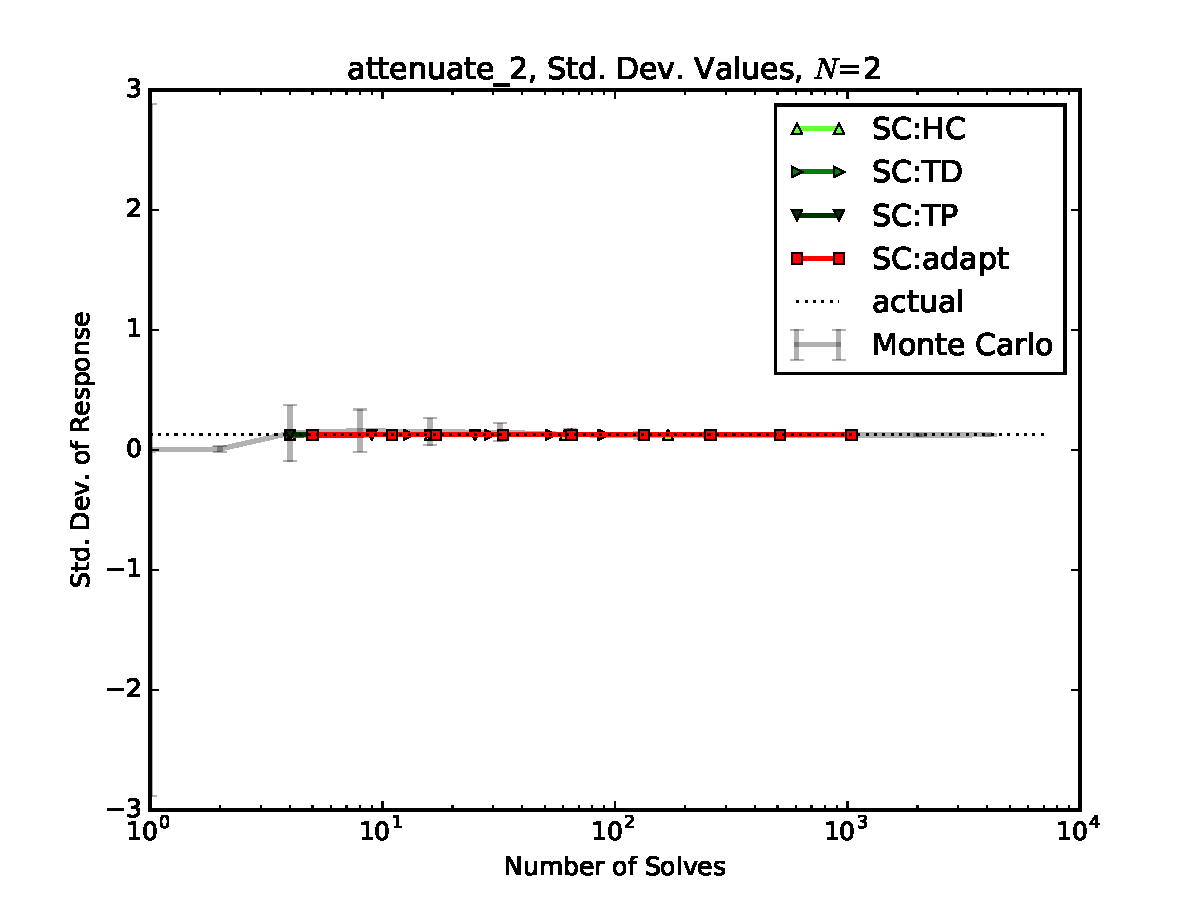
\includegraphics[width=0.7\linewidth]{anlmodels/attenuate_2_var_vals_nohdmr}
  \caption{Attenuation, $N=2$, Std. Dev. Values}
  \label{fig:attenuate var values 2}
\end{figure}

\begin{figure}[H]
  \centering
  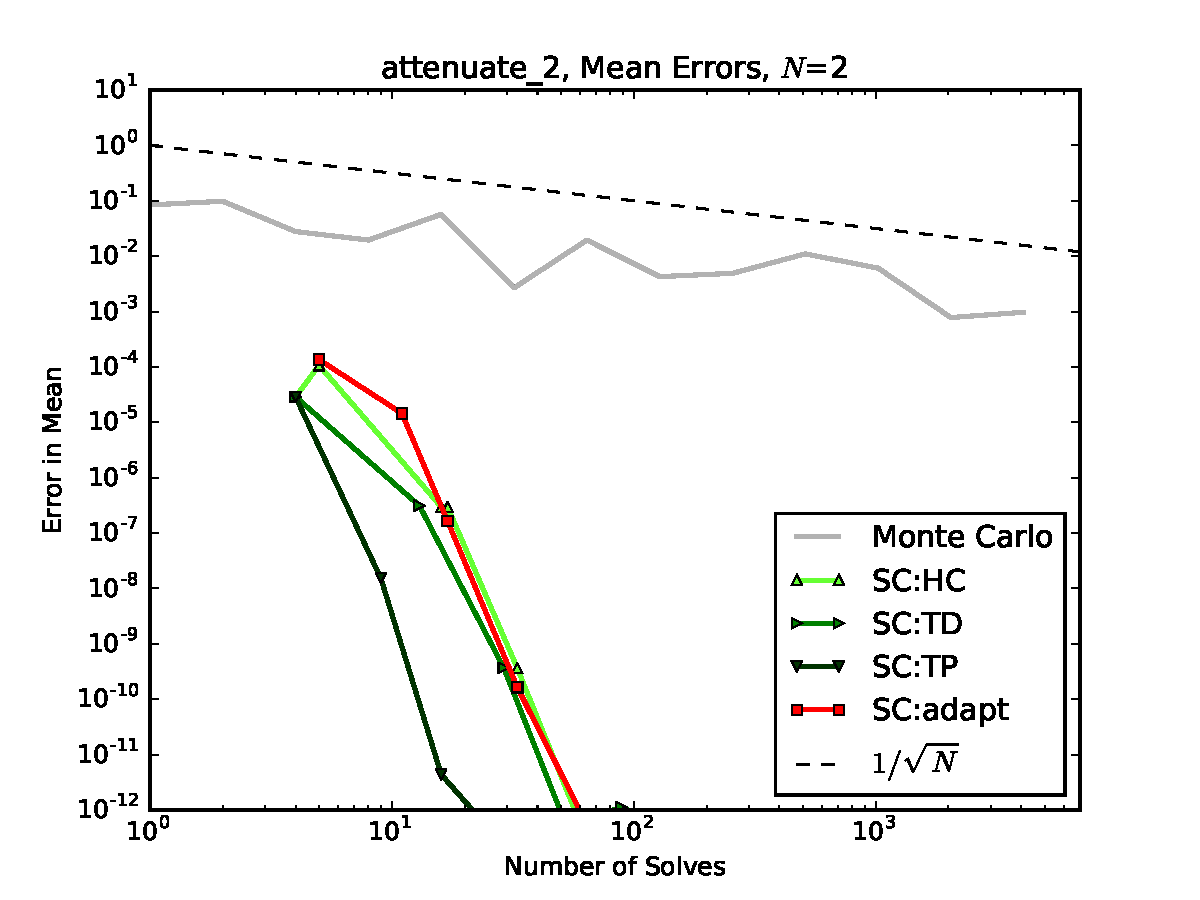
\includegraphics[width=0.7\linewidth]{anlmodels/attenuate_2_mean_errs_nohdmr}
  \caption{Attenuation, $N=2$, Mean Convergence}
  \label{fig:attenuate mean errors 2}
\end{figure}
\begin{figure}[H]
  \centering
  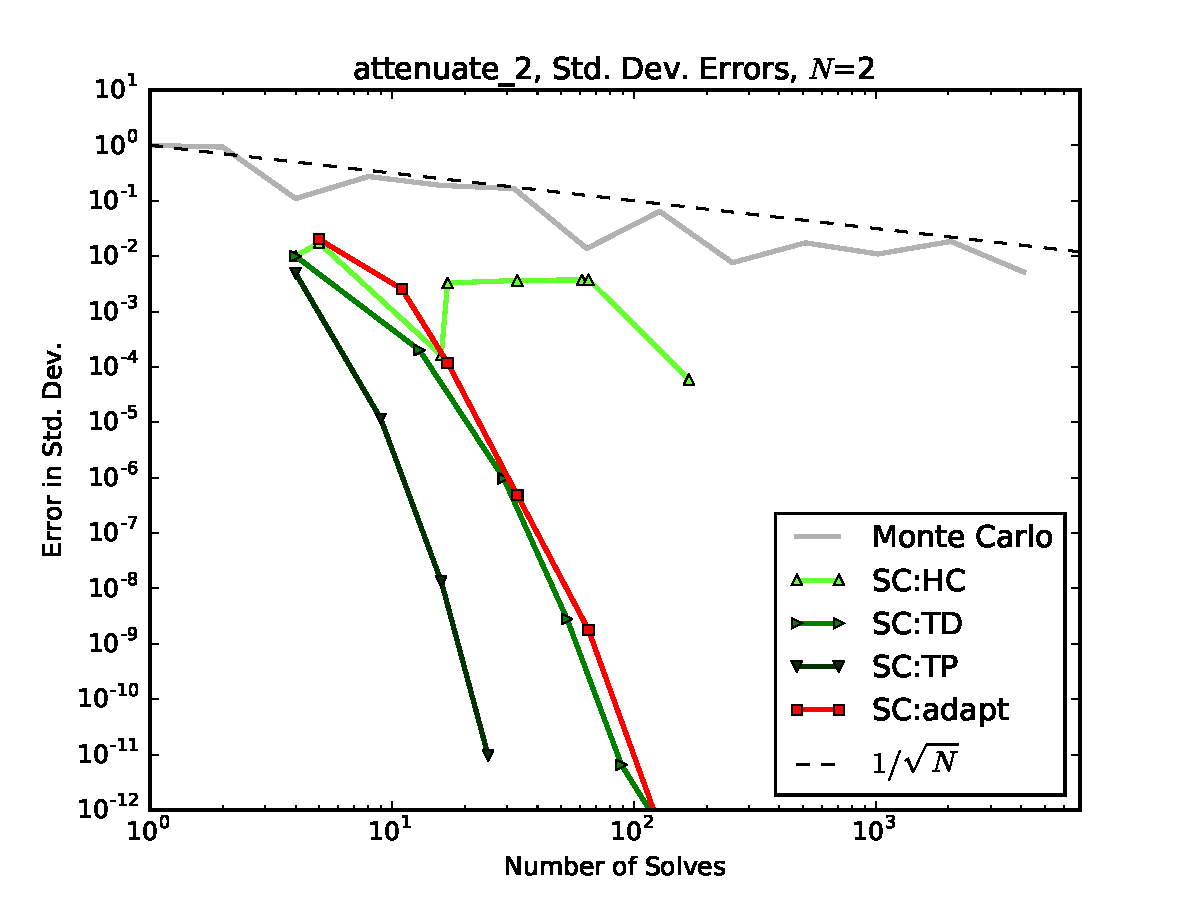
\includegraphics[width=0.7\linewidth]{anlmodels/attenuate_2_variance_errs_nohdmr}
  \caption{Attenuation, $N=2$, Std. Dev. Convergence}
  \label{fig:attenuate var errors 2}
\end{figure}


\subsection{4 Inputs}
As with the two-input case, all methods show good convergence on the mean, and only the Hyperbolic Cross
polynomials show poor performance for the standard deviation.  Interestingly, despite Tensor Product matching
the construction shape of the model well, both Total Degree and Adaptive perform quite similarly and converge
quite well.
\begin{figure}[H]
  \centering
  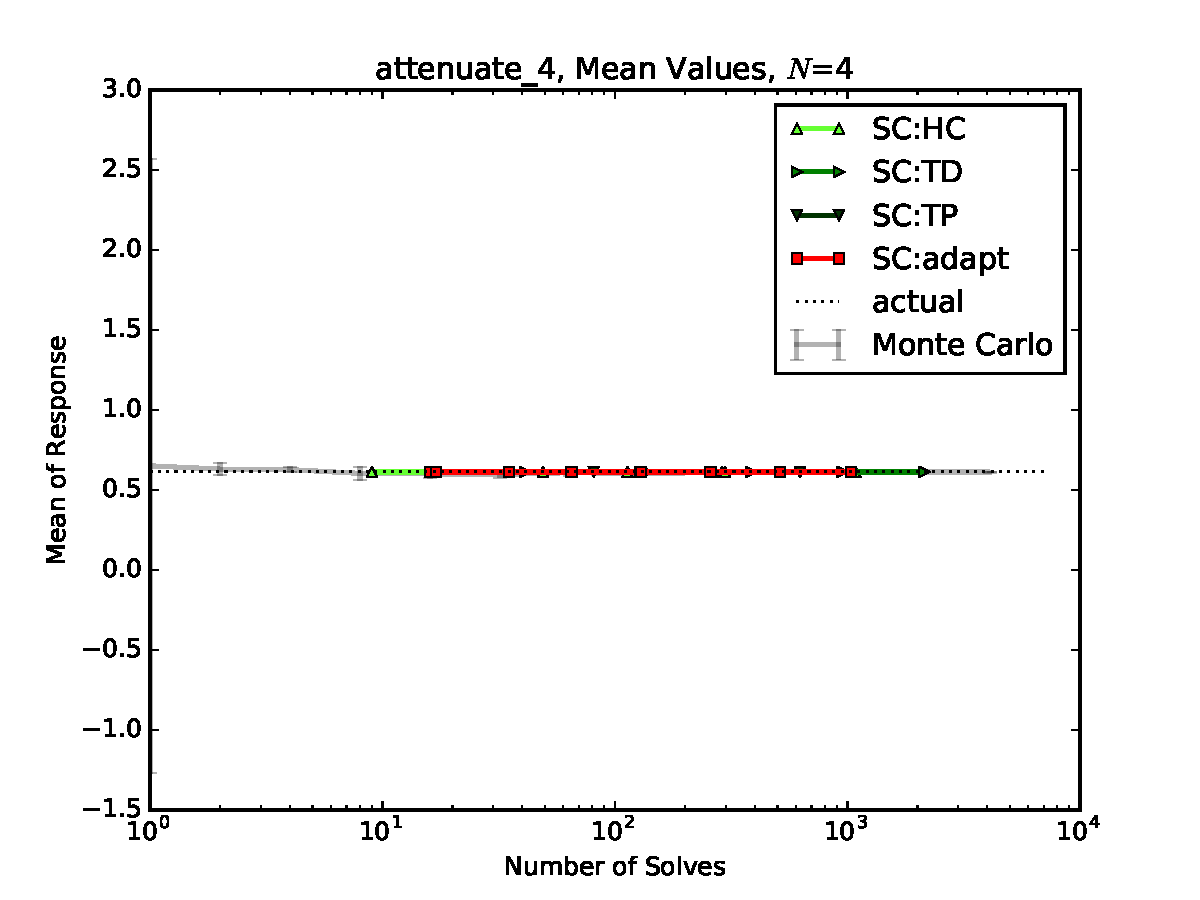
\includegraphics[width=0.7\linewidth]{anlmodels/attenuate_4_mean_vals_nohdmr}
  \caption{Attenuation, $N=4$, Mean Values}
  \label{fig:attenuate mean values 4}
\end{figure}
\begin{figure}[H]
  \centering
  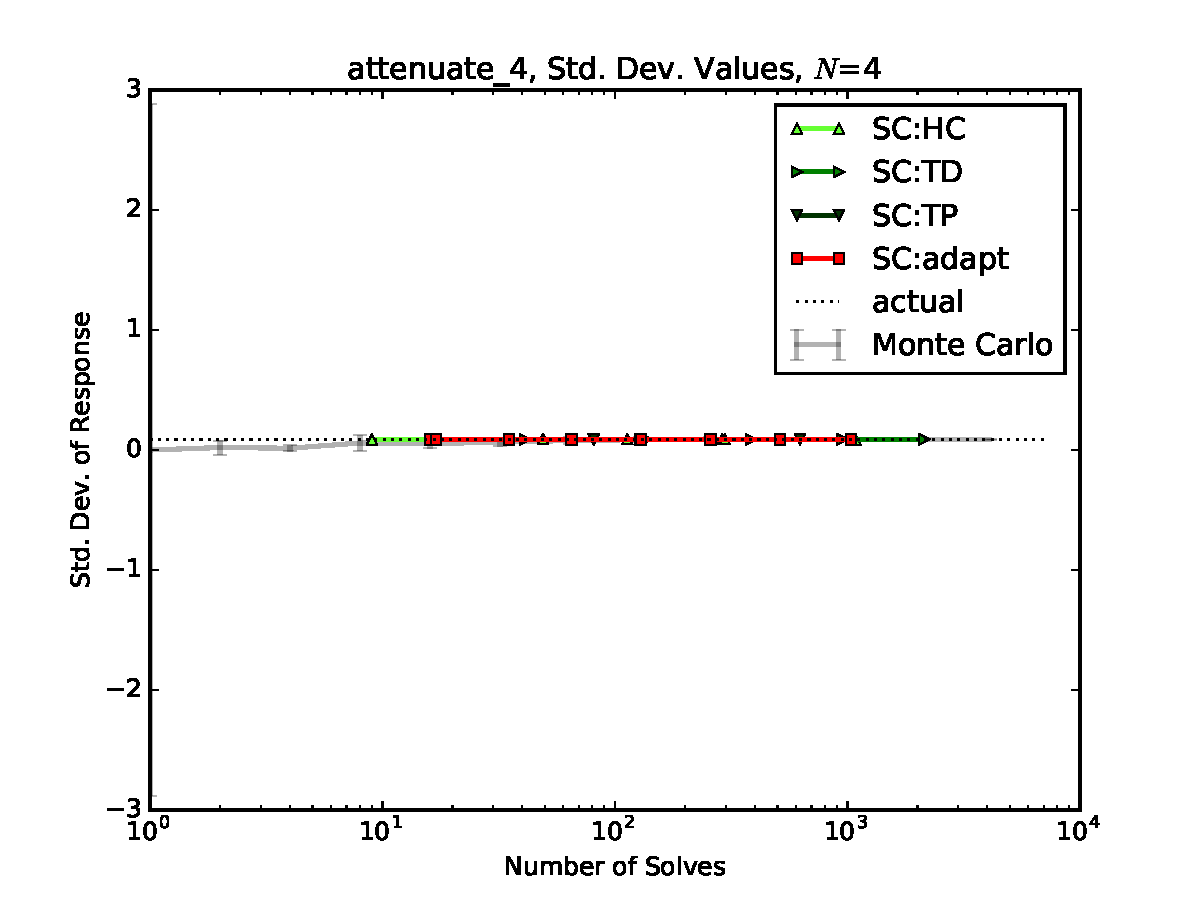
\includegraphics[width=0.7\linewidth]{anlmodels/attenuate_4_var_vals_nohdmr}
  \caption{Attenuation, $N=4$, Std. Dev. Values}
  \label{fig:attenuate var values 4}
\end{figure}

\begin{figure}[H]
  \centering
  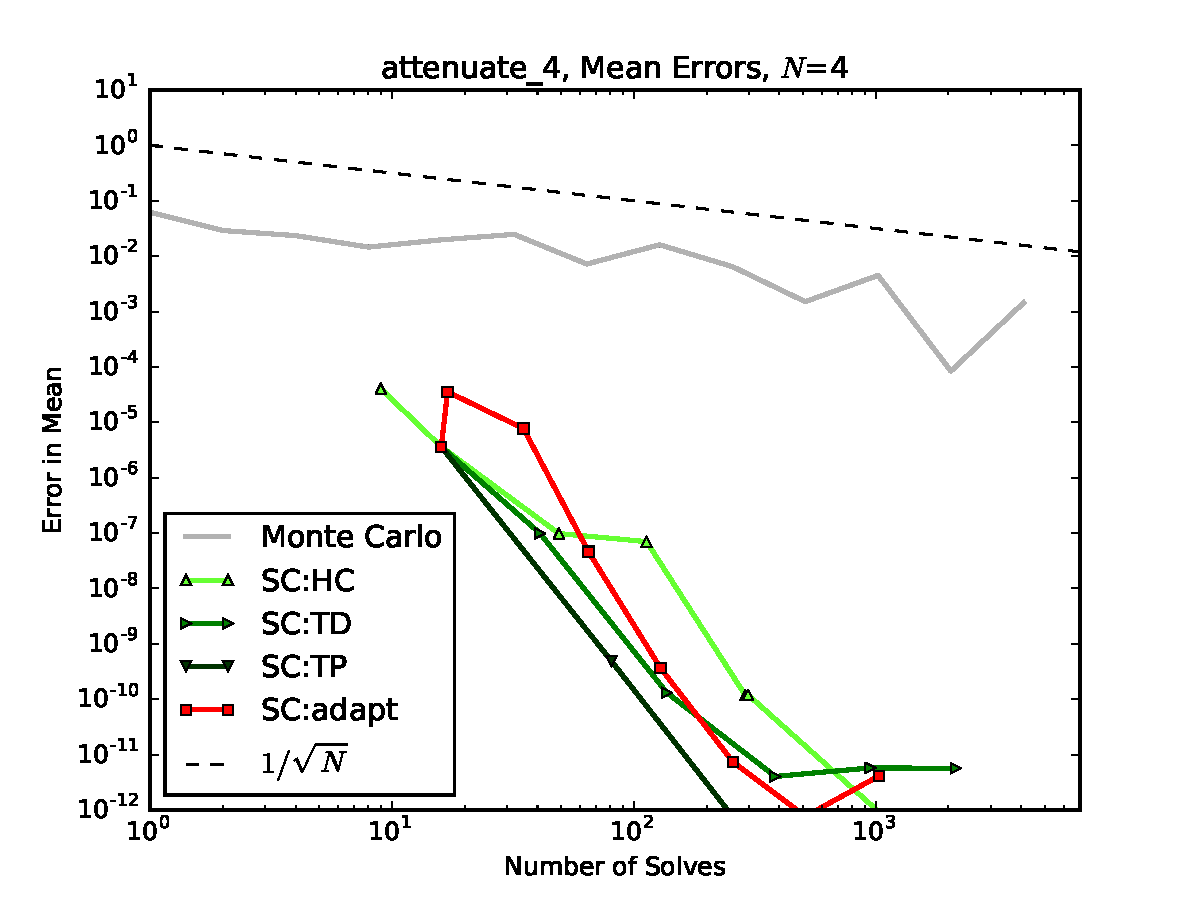
\includegraphics[width=0.7\linewidth]{anlmodels/attenuate_4_mean_errs_nohdmr}
  \caption{Attenuation, $N=4$, Mean Convergence}
  \label{fig:attenuate mean errors 4}
\end{figure}
\begin{figure}[H]
  \centering
  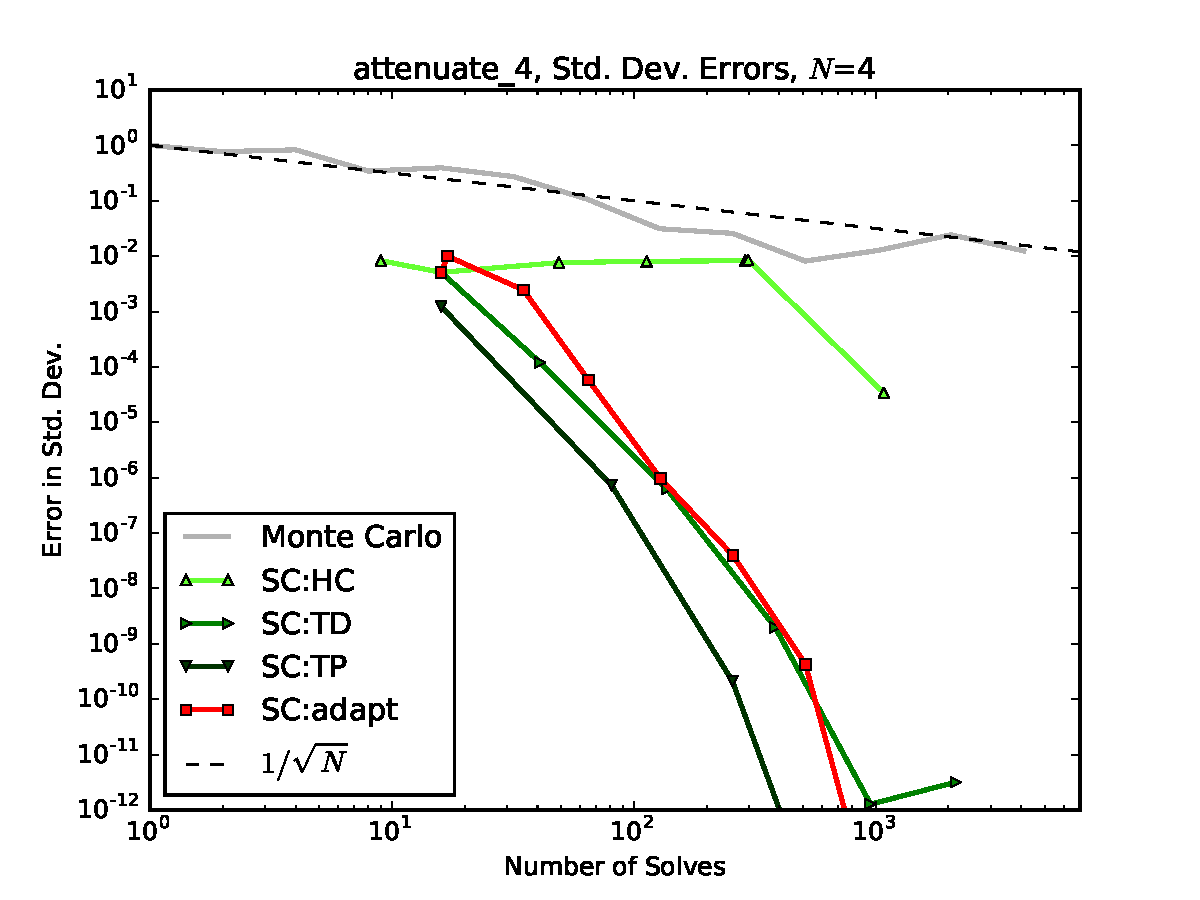
\includegraphics[width=0.7\linewidth]{anlmodels/attenuate_4_variance_errs_nohdmr}
  \caption{Attenuation, $N=4$, Std. Dev. Convergence}
  \label{fig:attenuate var errors 4}
\end{figure}

\subsection{6 Inputs}
The general trend in the two-input and four-input cases continues for six inputs, with one exception.  For six
inputs, the Adaptive method struggles to find the most suitable set of polynomials to include in the
expansion.  This is likely because of the large number of polynomial combinations available to consider 
with the larger input space.  If there is any tendency to inaccurately guess the path to take, this misstep is
likely to consider many times before the more accurate path is discovered.  Otherwise, exponential convergence
is still observed, but with a larger radius of curvature than the lower-dimension cases.
\begin{figure}[H]
  \centering
  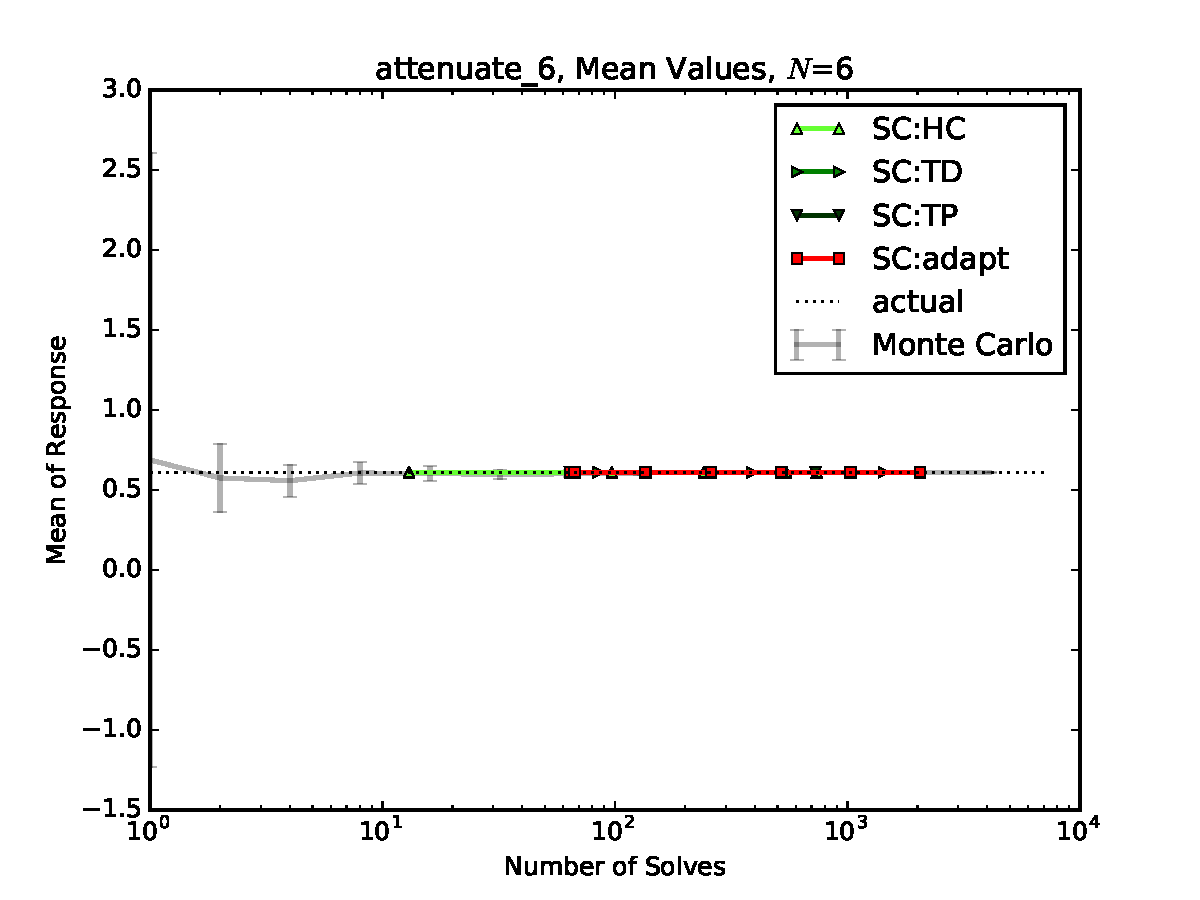
\includegraphics[width=0.7\linewidth]{anlmodels/attenuate_6_mean_vals_nohdmr}
  \caption{Attenuation, $N=6$, Mean Values}
  \label{fig:attenuate mean values 6}
\end{figure}
\begin{figure}[H]
  \centering
  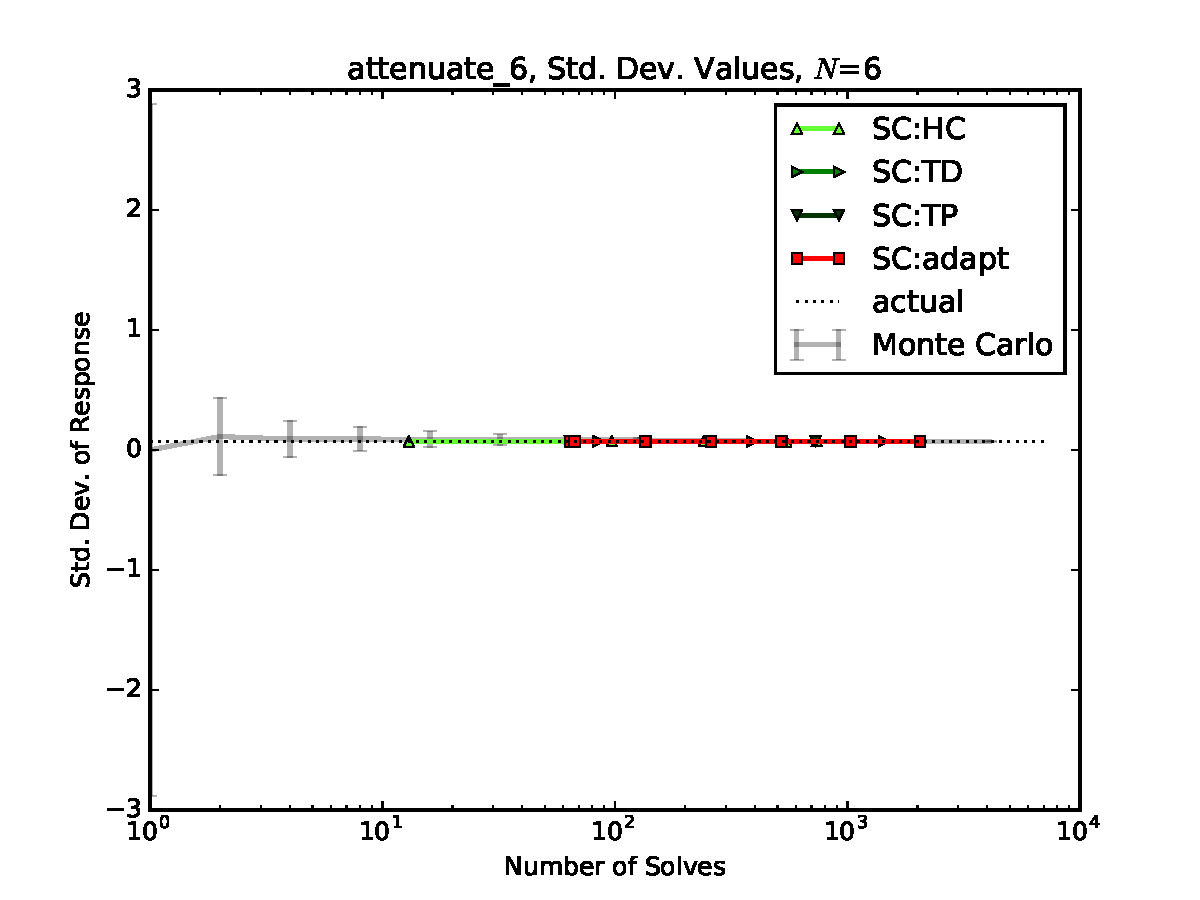
\includegraphics[width=0.7\linewidth]{anlmodels/attenuate_6_var_vals_nohdmr}
  \caption{Attenuation, $N=6$, Std. Dev. Values}
  \label{fig:attenuate var values 6}
\end{figure}

\begin{figure}[H]
  \centering
  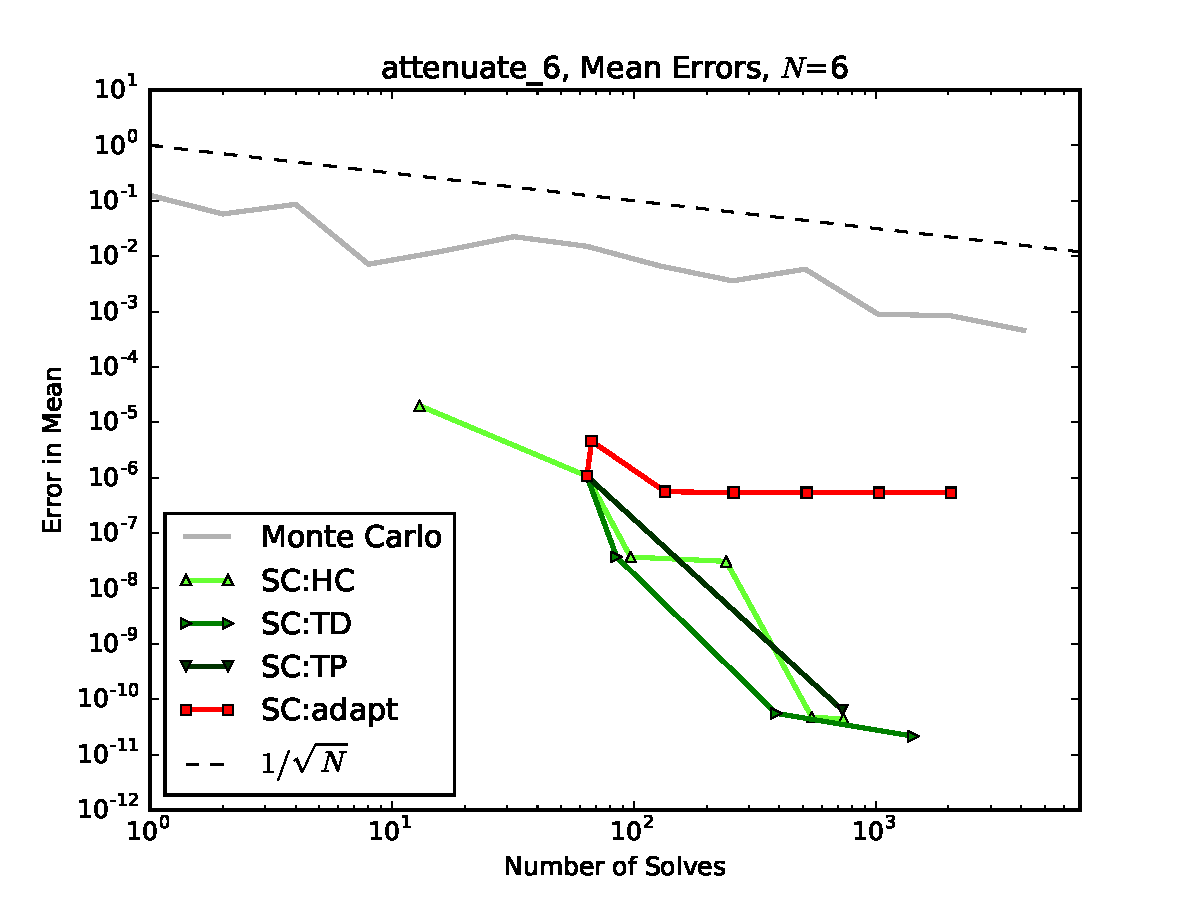
\includegraphics[width=0.7\linewidth]{anlmodels/attenuate_6_mean_errs_nohdmr}
  \caption{Attenuation, $N=6$, Mean Convergence}
  \label{fig:attenuate mean errors 6}
\end{figure}
\begin{figure}[H]
  \centering
  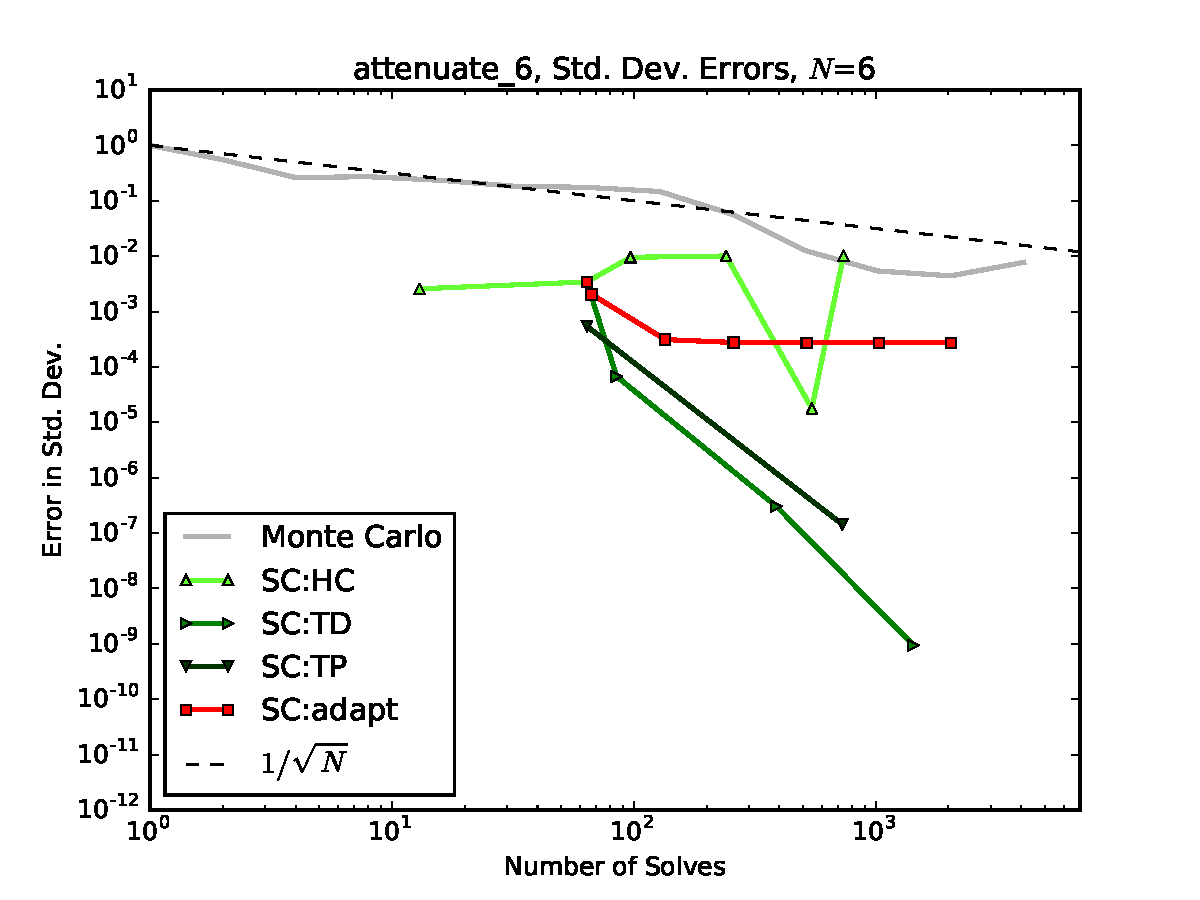
\includegraphics[width=0.7\linewidth]{anlmodels/attenuate_6_variance_errs_nohdmr}
  \caption{Attenuation, $N=6$, Std. Dev. Convergence}
  \label{fig:attenuate var errors 6}
\end{figure}


\section{Gauss Peak}
\subsection{Description}
Similar to the attenuation model, the Gaussian peak \cite{sfugenz} instead uses square arguments to the
exponential function.  A tuning parameter $a$ can also be used to change the peakedness of the
function.  Increased peakedness leads to more difficult polynomial representation.
A location parameter $\mu$ can be used to change the location of the peak.
The mathematical expression is
\begin{equation}
  u(Y) = \exp\qty(-\sum_{n=1}^N a^2\qty(y_n-\mu)^2).
\end{equation}
We allow each $y_n$ to vary uniformly on [0,1] and set peakedness to $a=3$, with the center
of the peak at (0.5,0.5).
The two-dimensional representation of this function is given in Figure \ref{fig: gauss peak}.
\begin{figure}[htb]
  \centering
  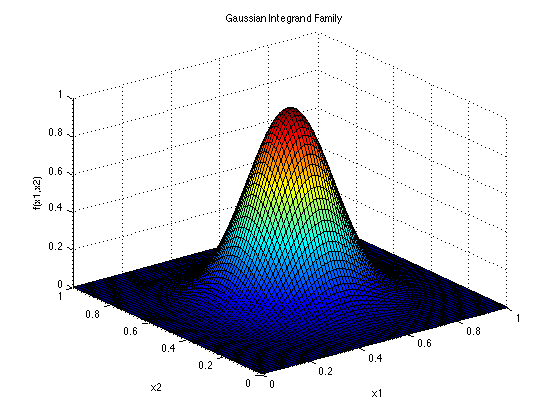
\includegraphics[width=0.7\linewidth]{anlmodels/gaussian}
  \caption{Gaussian Peak \cite{sfu}}
  \label{fig: gauss peak}
\end{figure}
A summary of analytic statistics is given in Table \ref{tab:gausspeak moments}.

\begin{table}[H]
  \centering
  \begin{tabular}{c|c}
    Statistic & Expression \\ \hline
    Mean & $\qty(\frac{\sqrt{\pi}}{2a}\qty(\erf(a\mu)+\erf(a-a\mu)))^N$ \\
    Variance & $\qty(\frac{\sqrt{\pi/2}}{2a}\qty(\erf(a\mu\sqrt{2})-\erf(a\sqrt{2}(1-\mu))))^N - 
        \qty(\frac{\sqrt{\pi}}{2a}\qty(\erf(a\mu)+\erf(a-a\mu)))^{2N}$
  \end{tabular}
  \caption{Analytic Expressions for Gaussian Peak Case}
  \label{tab:gausspeak moments}
\end{table}
This case offers particular challenge because of its Taylor development, which only includes even powers of
the uncertain parameters.  This suggests added difficulty in successive representation, especially for an
adaptive algorithm.

\subsection{Discussion}
As for the attenuation model, this model is best understood in light of its polynomial representation, given
by the Taylor expansion (for example for $\mu=0$ about $y=0$):
\begin{equation}
e^{-a^2y^2} = 1 - a^2y^2 + \frac{(a^2y^2)^2}{2} - \frac{(a^2y^2)^3}{6} + \frac{(a^2y^2)^4}{24} - \frac{(a^2y^2)^5}{120} + \mathcal{O}(y^6).
\end{equation}
Because this model's coefficient $a=3$, it serves to balance against the cross-term preference in the product
of two terms, instead of exacerbating it as in the attenuation model.  Because of this, terms with the same total
effective polynomial order are more nearly equal in importance.  In addition, because of the peaking term,
more polynomials are required to accurately represent this model.  As a result, we observe errors to be larger
for all methods, and the tensor product to have reduced error in comparison to the other methods, all when
compared to the attenuation model.

\subsection{3 Inputs}
For this smaller input space, we see good exponential convergence on the mean for the Hyperbolic Cross, Total
Degree, and Tensor Product index sets.  However, the adaptive method fails entirely.  This is because none of
the first-order polynomials have any contribution even when integrated coarsely; as a result, the adaptive
algorithm is duped into believing it is converged.  This same behavior is seen for the five-input case as
well.  As expected, the standard deviation shows poorer performance for all three methods than the mean; in
fact, only the Tensor Product is clearly converging for the standard deviation even with only three inputs.
This demonstrates the challenge of this model to be represented well with polynomials.
\begin{figure}[H]
  \centering
  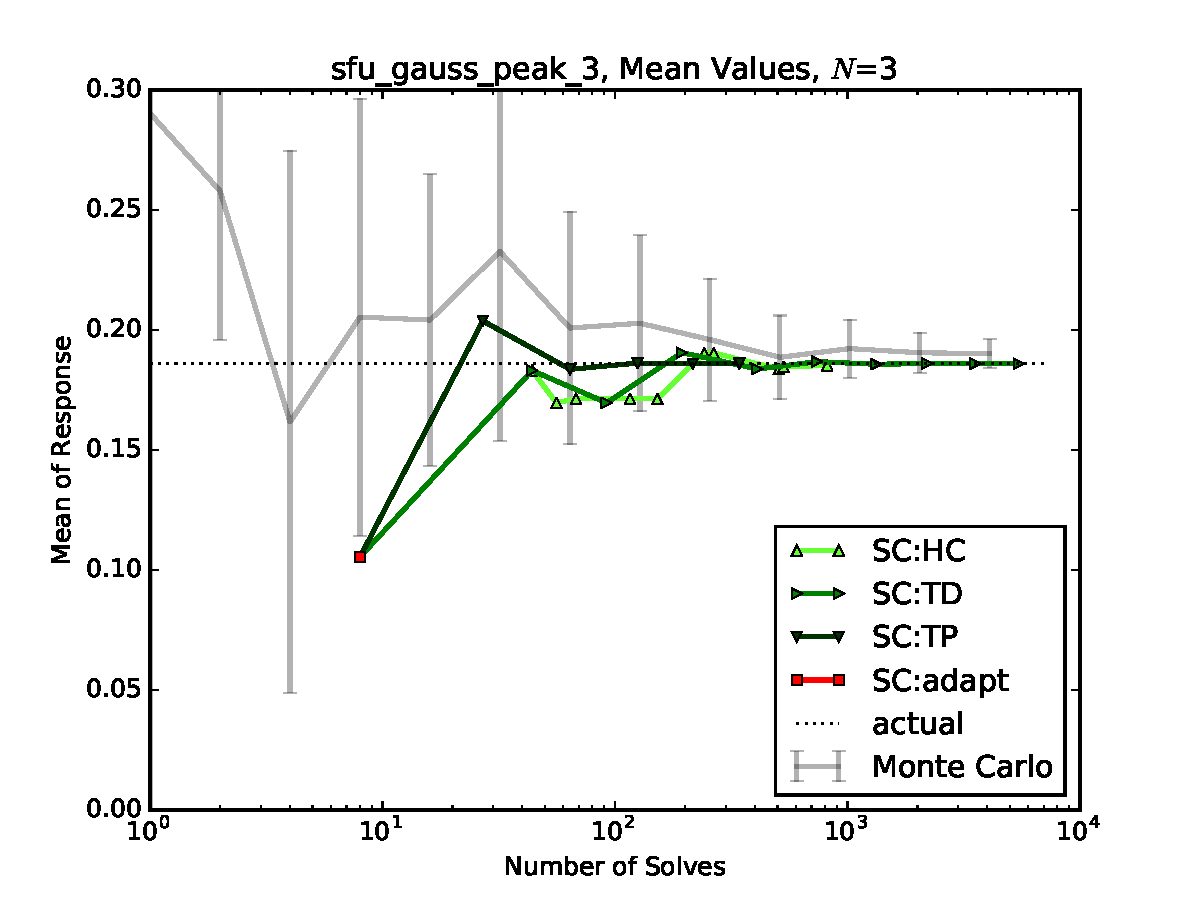
\includegraphics[width=0.7\linewidth]{anlmodels/sfu_gauss_peak_3_mean_vals_nohdmr}
  \caption{Gauss Peak, $N=3$, Mean Values}
  \label{fig:gauss peak mean values 3}
\end{figure}
\begin{figure}[H]
  \centering
  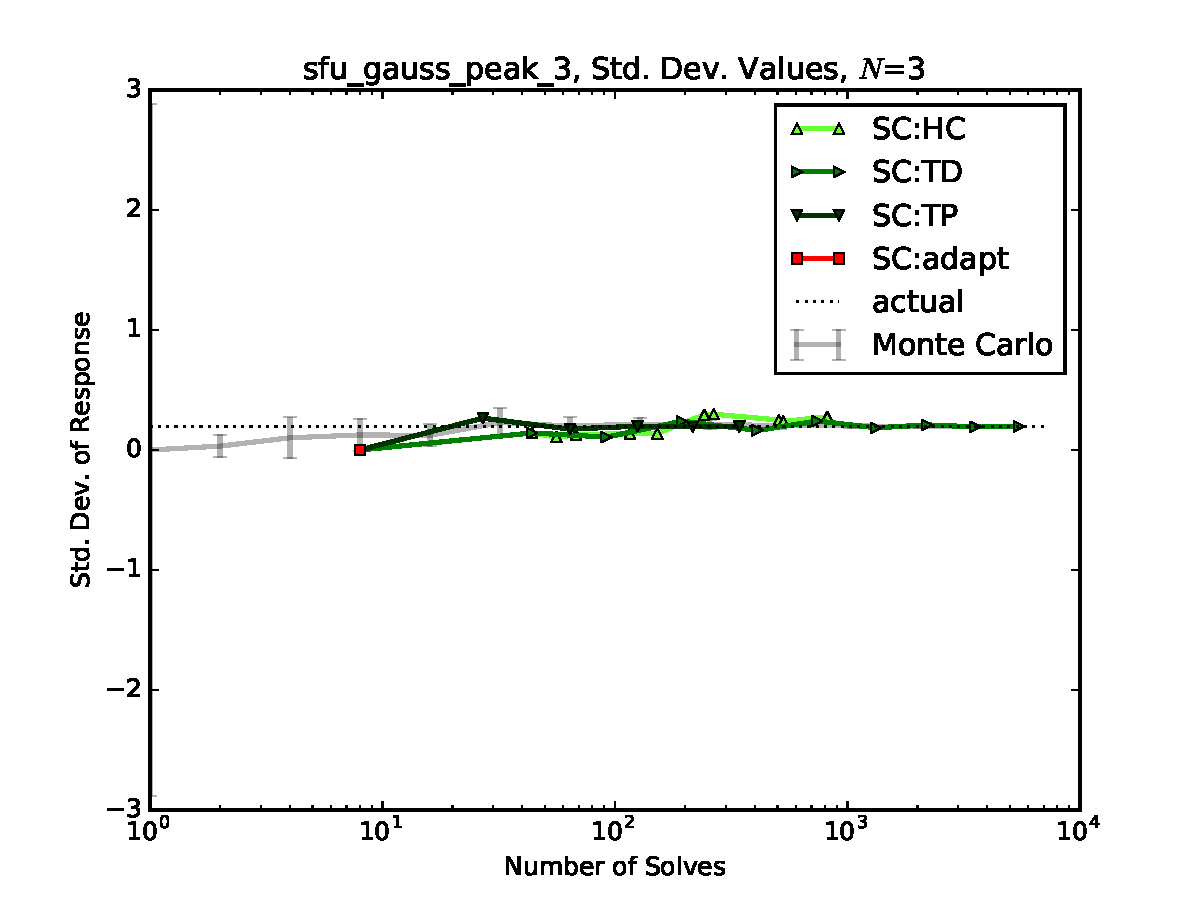
\includegraphics[width=0.7\linewidth]{anlmodels/sfu_gauss_peak_3_var_vals_nohdmr}
  \caption{Gauss Peak, $N=3$, Std. Dev. Values}
  \label{fig:gauss peak var values 3}
\end{figure}

\begin{figure}[H]
  \centering
  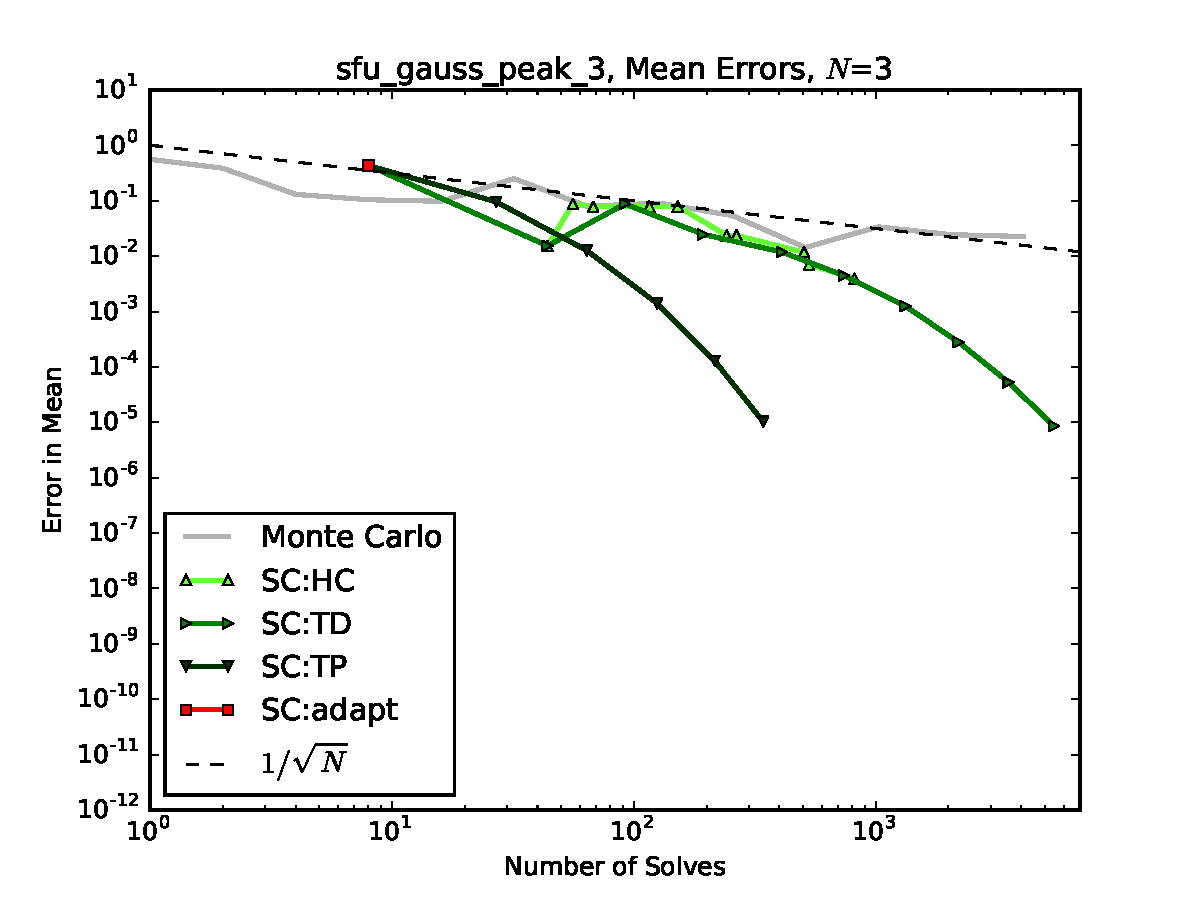
\includegraphics[width=0.7\linewidth]{anlmodels/sfu_gauss_peak_3_mean_errs_nohdmr}
  \caption{Gauss Peak, $N=3$, Mean Convergence}
  \label{fig:gauss peak mean errors 3}
\end{figure}
\begin{figure}[H]
  \centering
  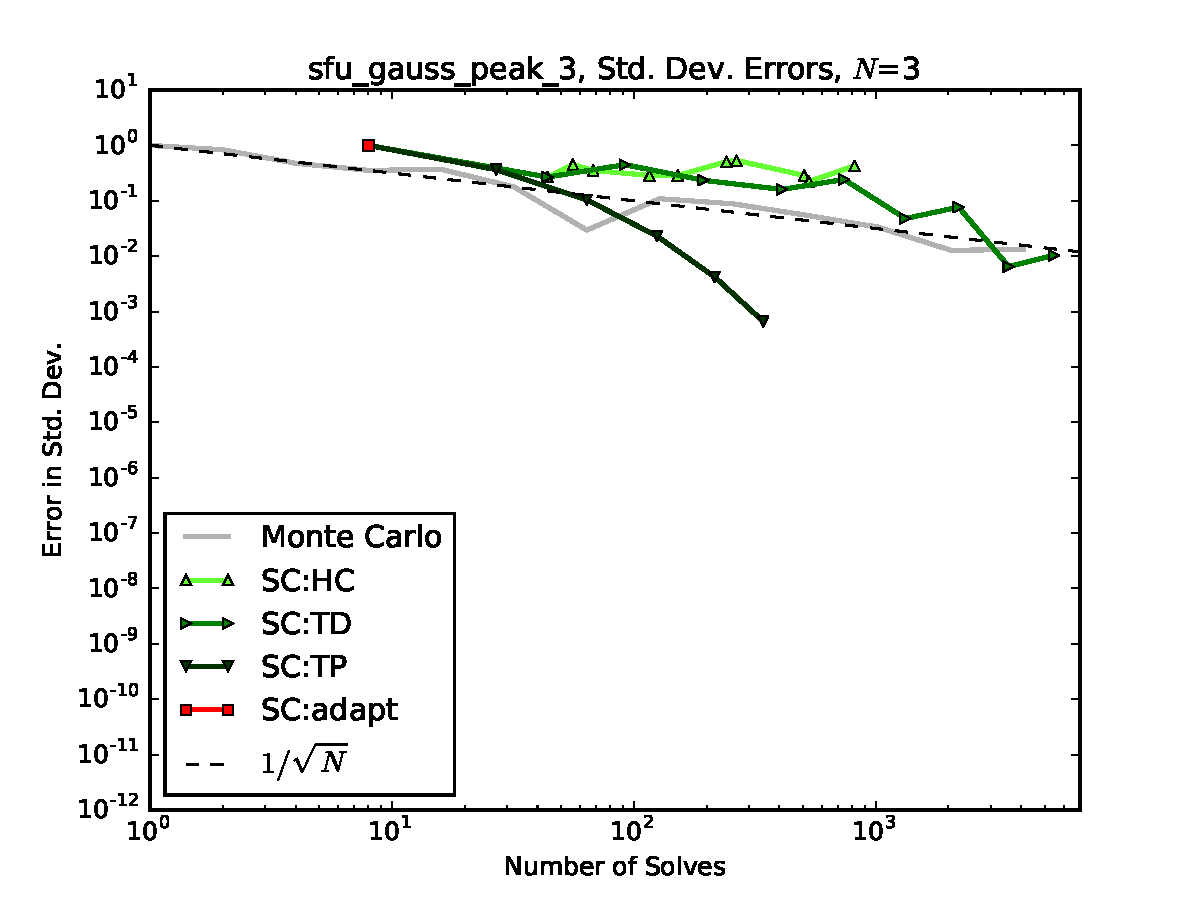
\includegraphics[width=0.7\linewidth]{anlmodels/sfu_gauss_peak_3_variance_errs_nohdmr}
  \caption{Gauss Peak, $N=3$, Std. Dev. Convergence}
  \label{fig:gauss peak var errors 3}
\end{figure}

\subsection{5 Inputs}
The same trends are observed for five inputs as for three, but with poorer convergence in all methods.  While
it appears there is some convergence benefits in the collocation methods, for up to 1000 computation solves
there is little advantage over Monte Carlo sampling.
\begin{figure}[H]
  \centering
  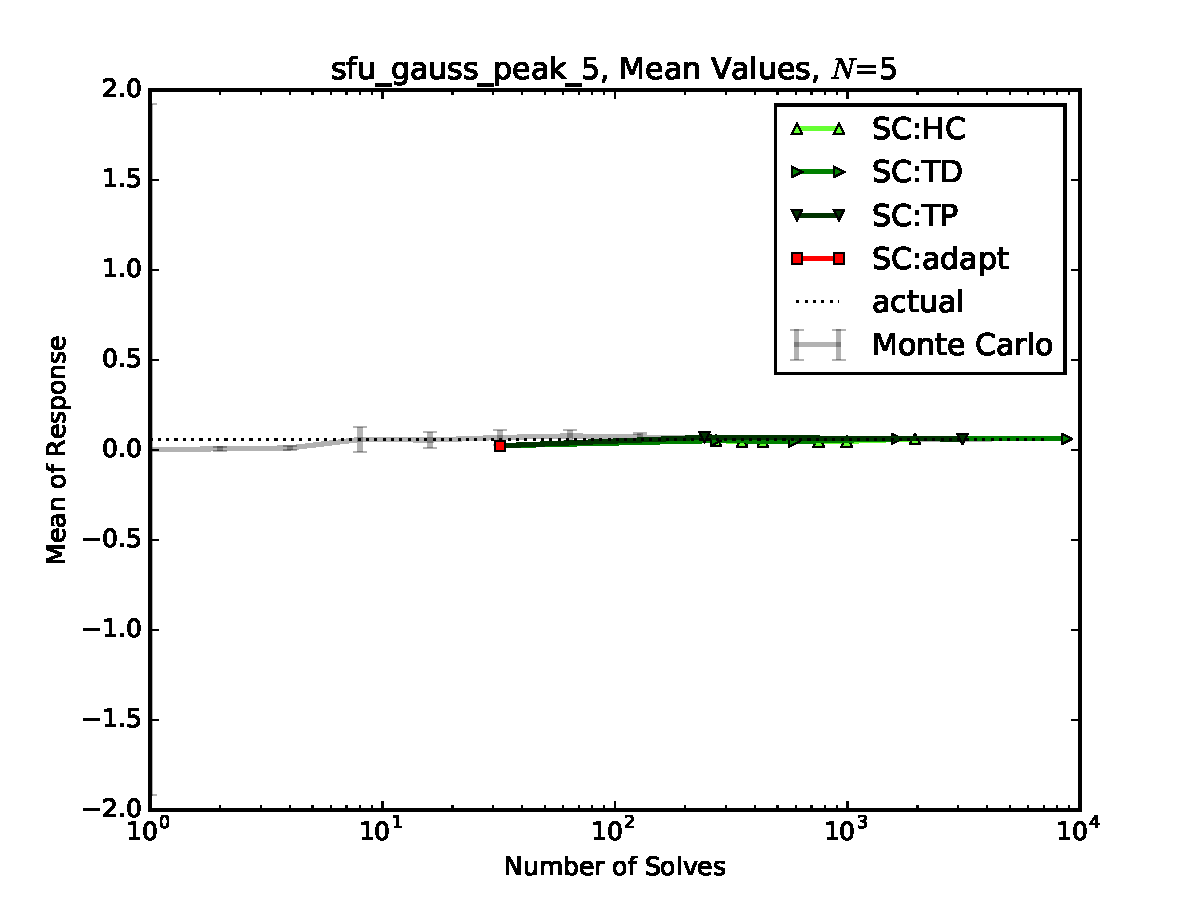
\includegraphics[width=0.7\linewidth]{anlmodels/sfu_gauss_peak_5_mean_vals_nohdmr}
  \caption{Gauss Peak, $N=5$, Mean Values}
  \label{fig:gauss peak mean values 5}
\end{figure}
\begin{figure}[H]
  \centering
  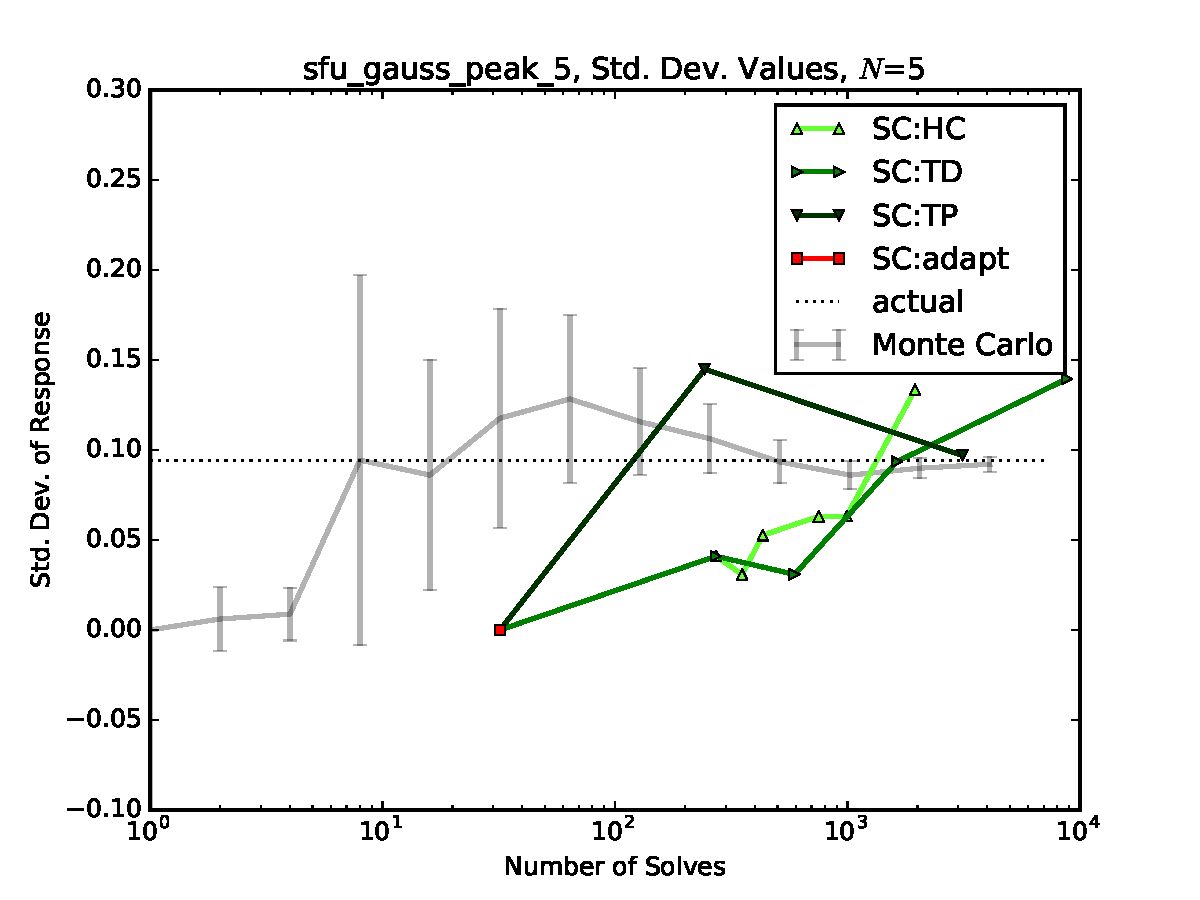
\includegraphics[width=0.7\linewidth]{anlmodels/sfu_gauss_peak_5_var_vals_nohdmr}
  \caption{Gauss Peak, $N=5$, Std. Dev. Values}
  \label{fig:gauss peak var values 5}
\end{figure}

\begin{figure}[H]
  \centering
  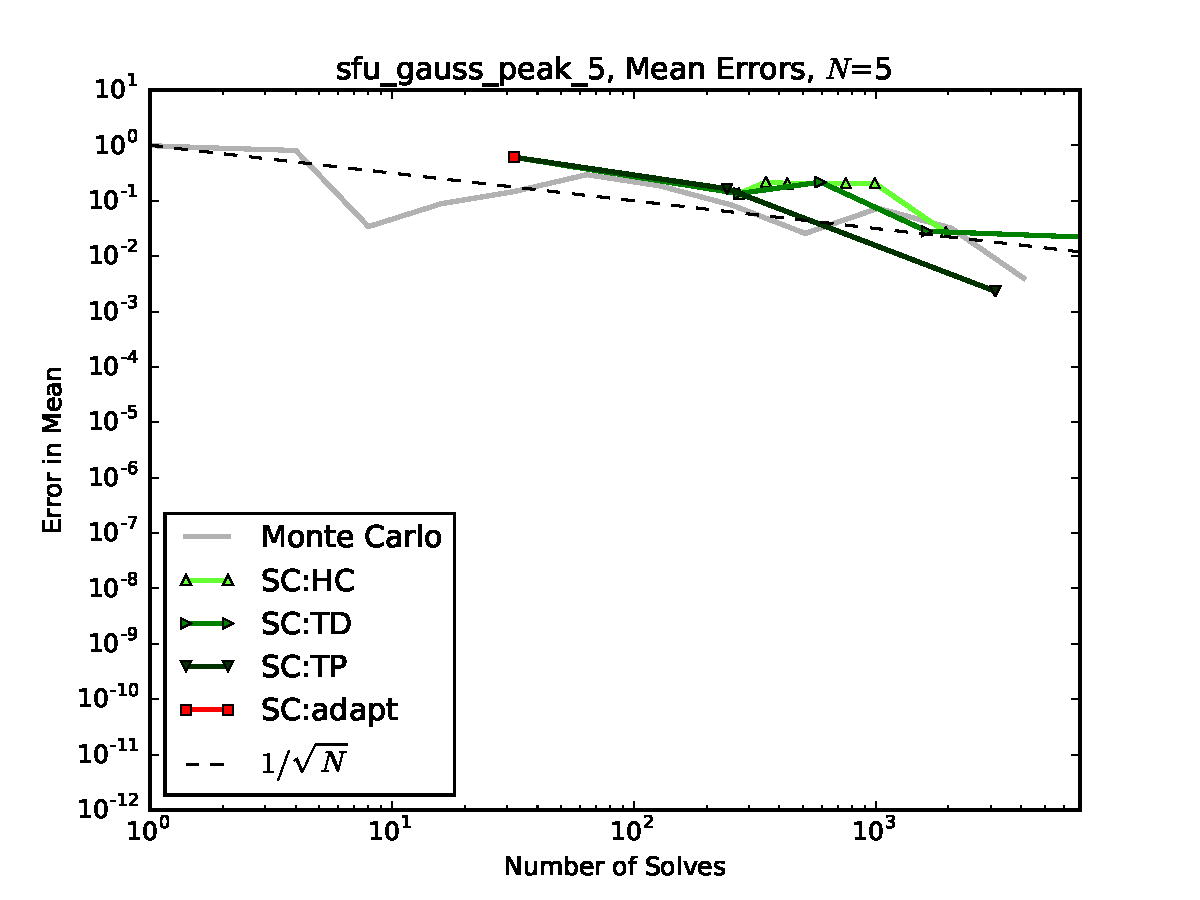
\includegraphics[width=0.7\linewidth]{anlmodels/sfu_gauss_peak_5_mean_errs_nohdmr}
  \caption{Gauss Peak, $N=5$, Mean Convergence}
  \label{fig:gauss peak mean errors 5}
\end{figure}
\begin{figure}[H]
  \centering
  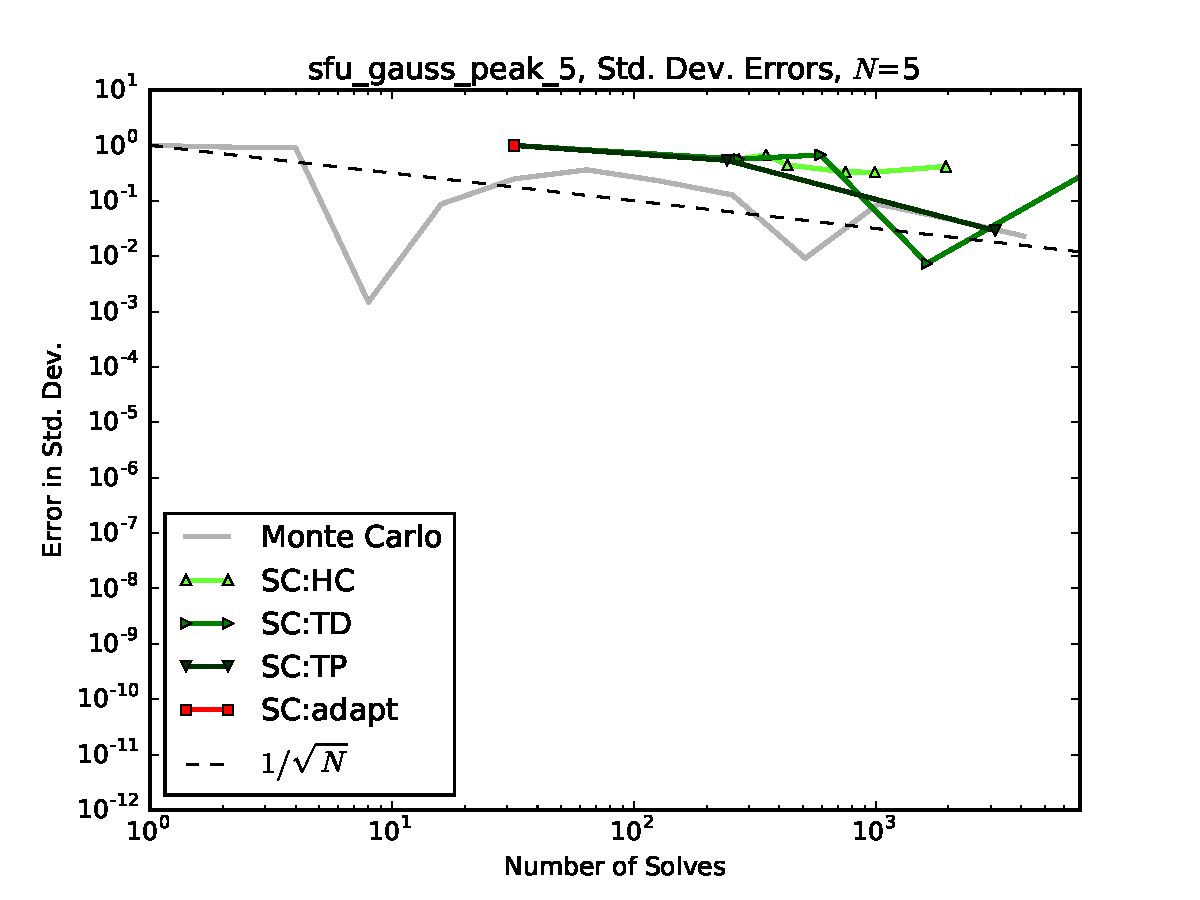
\includegraphics[width=0.7\linewidth]{anlmodels/sfu_gauss_peak_5_variance_errs_nohdmr}
  \caption{Gauss Peak, $N=5$, Std. Dev. Convergence}
  \label{fig:gauss peak var errors 5}
\end{figure}




\section{Ishigami}
\subsection{Description}
The Ishigami function \cite{ishigami} is a commonly-used function in performing sensitivity analysis.  It is
given by
\begin{equation}
  u(Y) = \sin{y_1} + a\sin^2{y_2} + b y_3^4\sin(y_1).
\end{equation}
In our case, we will use $a=7$ and $b=0.1$ as in \cite{ishigami2}.
The graphical representation of this function is given in Figure \ref{fig: ishigami}, with the three axes
as the three inputs and the color map as the function values ranging approximately from -10.74 to 17.74.
\begin{figure}[htb]
  \centering
  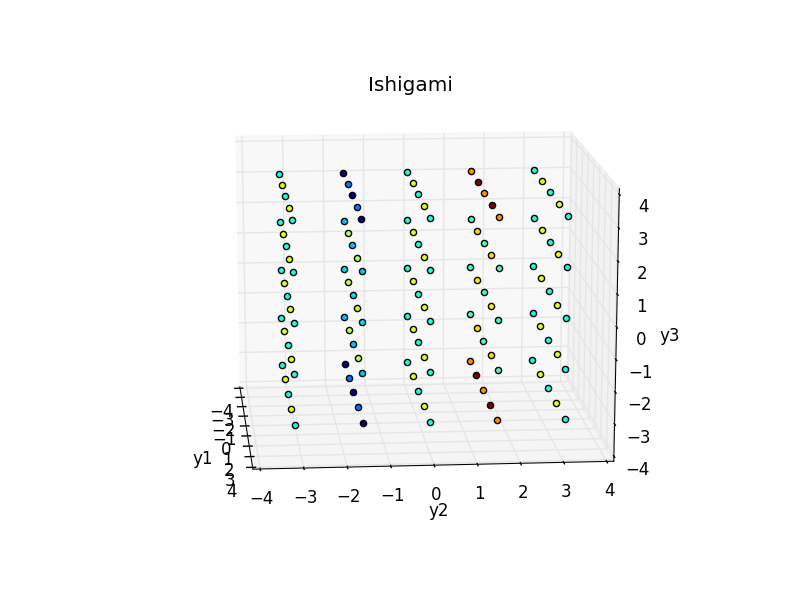
\includegraphics[width=0.7\linewidth]{anlmodels/ishigami}
  \caption{Ishigami Model}
  \label{fig: ishigami}
\end{figure}
In particular interest for this model are
its strong nonlinearity and lack of independence for $y_3$, as it only appears in conjunction with $y_1$.  The
analytic statistics of interest for this model are in Table \ref{tab:ishigami moments}, where $D_n$ is the
partial variance contributed by $y_n$ and Sobol sensitivities $\mathcal{S}_n$ are obtained by dividing $D_n$
by the total variance.

\begin{table}[H]
  \centering
  \begin{tabular}{c|c|c}
  Statistic & Expression & Approx. Value \\\hline
  Mean & $\frac{7}{2}$ & 3.5 \\
  Variance & $\frac{a^2}{8} + \frac{b\pi^4}{5} + \frac{b^2\pi^8}{18} + \frac{1}{2}$ & 13.84459 \\
  $D_1$ & $\frac{b\pi^4}{5} + \frac{b^2\pi^8}{50} + \frac{1}{2} $ &  4.34589 \\
  $D_2$ & $\frac{a^2}{8}$ & 6.125 \\
  $D_{1,3}$ & $\frac{8b^2\pi^8}{225}$ & 3.3737 \\
  $D_3,D_{1,2},D_{2,3},D_{1,2,3}$ & 0 & 0
  \end{tabular}
  \caption{Analytic Expressions for Ishigami Case}
  \label{tab:ishigami moments}
\end{table}


\subsection{Discussion}
The Ishigami function is sinusoidal in $y_1$ and $y_2$.  Because the sine function is exclusively odd, this presents
a similar challenge as previous models to adaptive methods, at least for these two dimensions.  $y_3$, however, only
appears as a fourth-order coefficient to the sine of $y_1$, which makes for a relationship that is difficult for the
polynomial representations to capture.  For this model, there is no flexibility in the dimensionality of the
input space; we show the only case ($N=3$) here.

\subsection{3 Inputs}
For the mean we see good convergence for the three static methods, and surprisingly good convergence for the
Hyperbolic Cross polynomials.  Because the two dominant parameters are largely independent, the polar focus of
the Hyperbolic Cross set captures the essential components with less computation than the other two static
methods.  The adaptive method, as predicted, struggles to find any important polynomials before finding false
convergence.

For the standard deviation, however, we see significant divergence for both the Hyperbolic Cross and Adaptive
methods.  Despite some oscillations, however, we do see exponential convergence for both the Tensor Product
and Total Degree methods.  Despite this, marked improvements over Monte Carlo are not distinct until near 1000
computational solves, despite the small input space.
\begin{figure}[H]
  \centering
  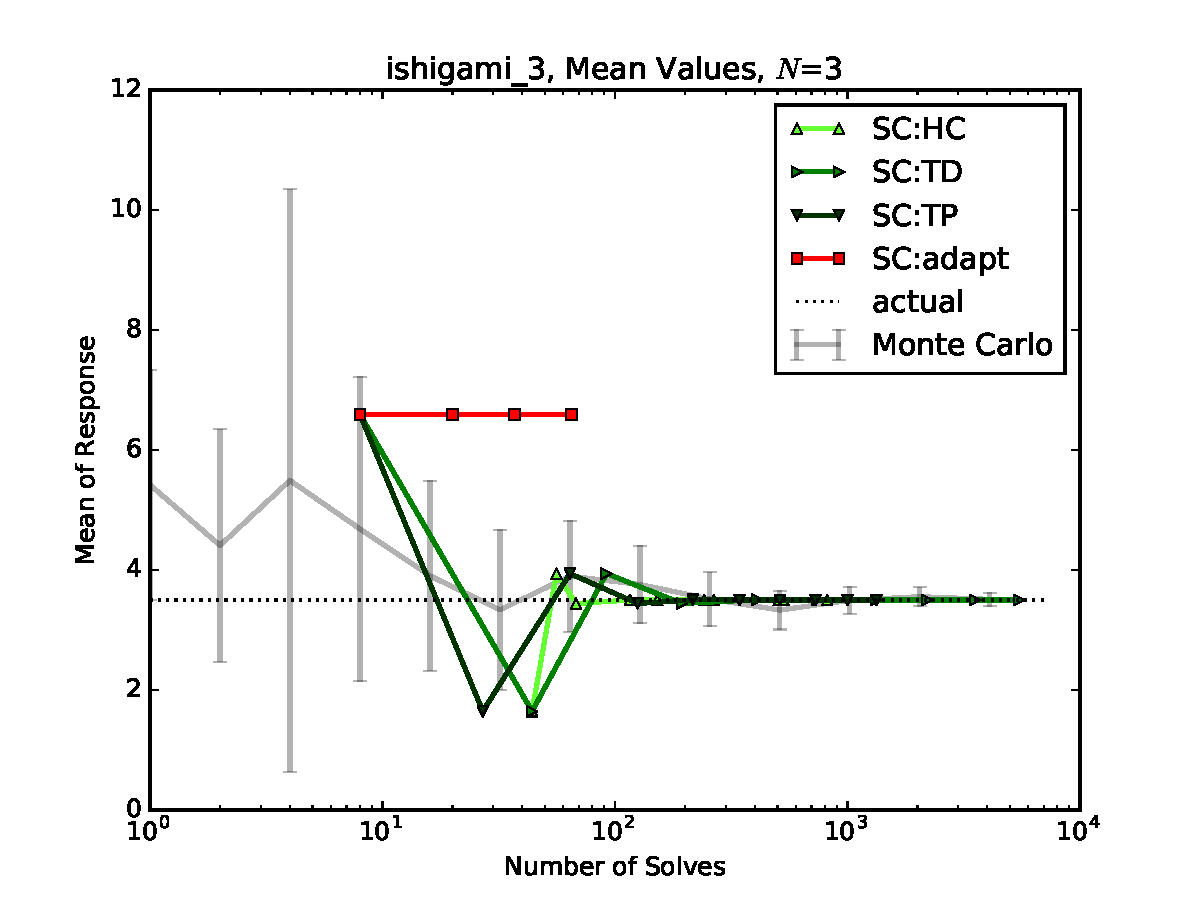
\includegraphics[width=0.7\linewidth]{anlmodels/ishigami_3_mean_vals_nohdmr}
  \caption{Ishigami, $N=3$, Mean Values}
  \label{fig:ishigami mean values 3}
\end{figure}
\begin{figure}[H]
  \centering
  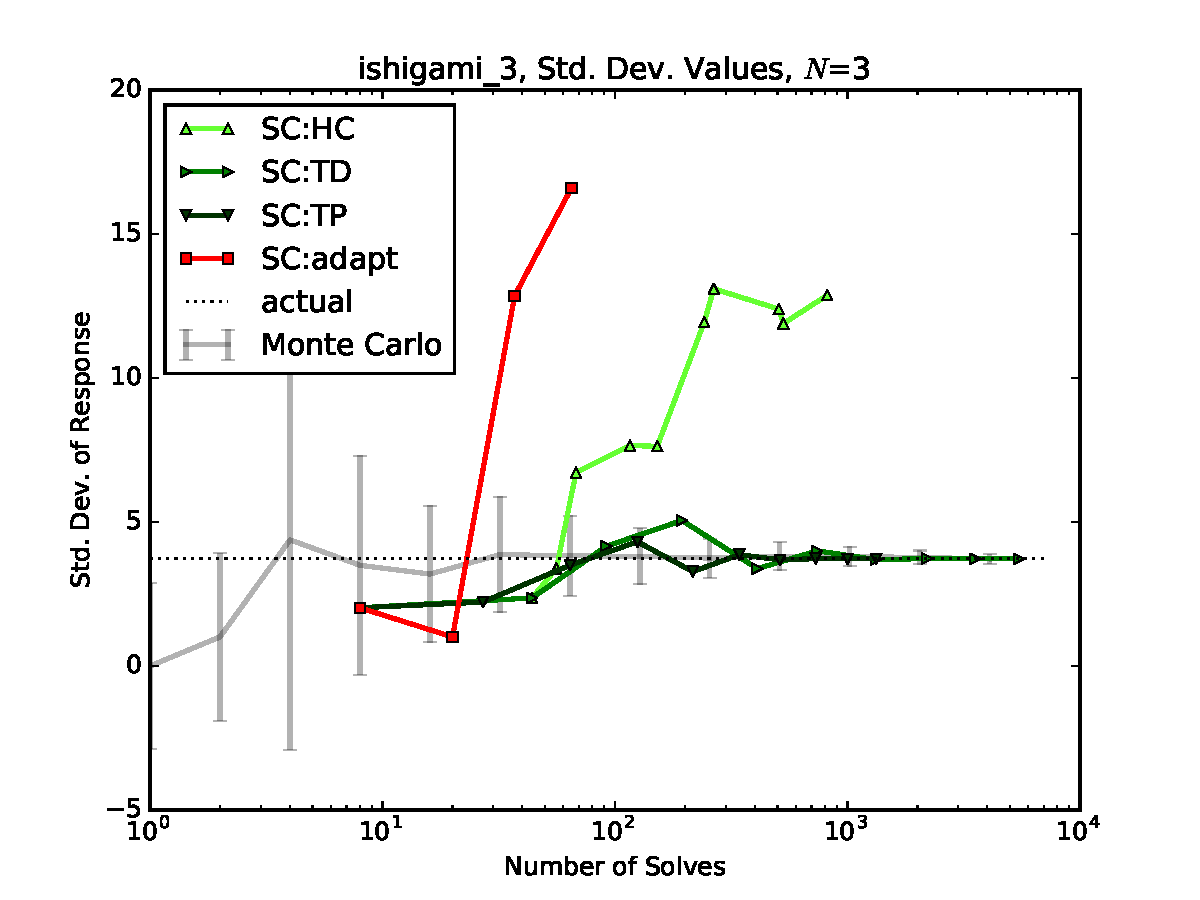
\includegraphics[width=0.7\linewidth]{anlmodels/ishigami_3_var_vals_nohdmr}
  \caption{Ishigami, $N=3$, Std. Dev. Values}
  \label{fig:ishigami var values 3}
\end{figure}

\begin{figure}[H]
  \centering
  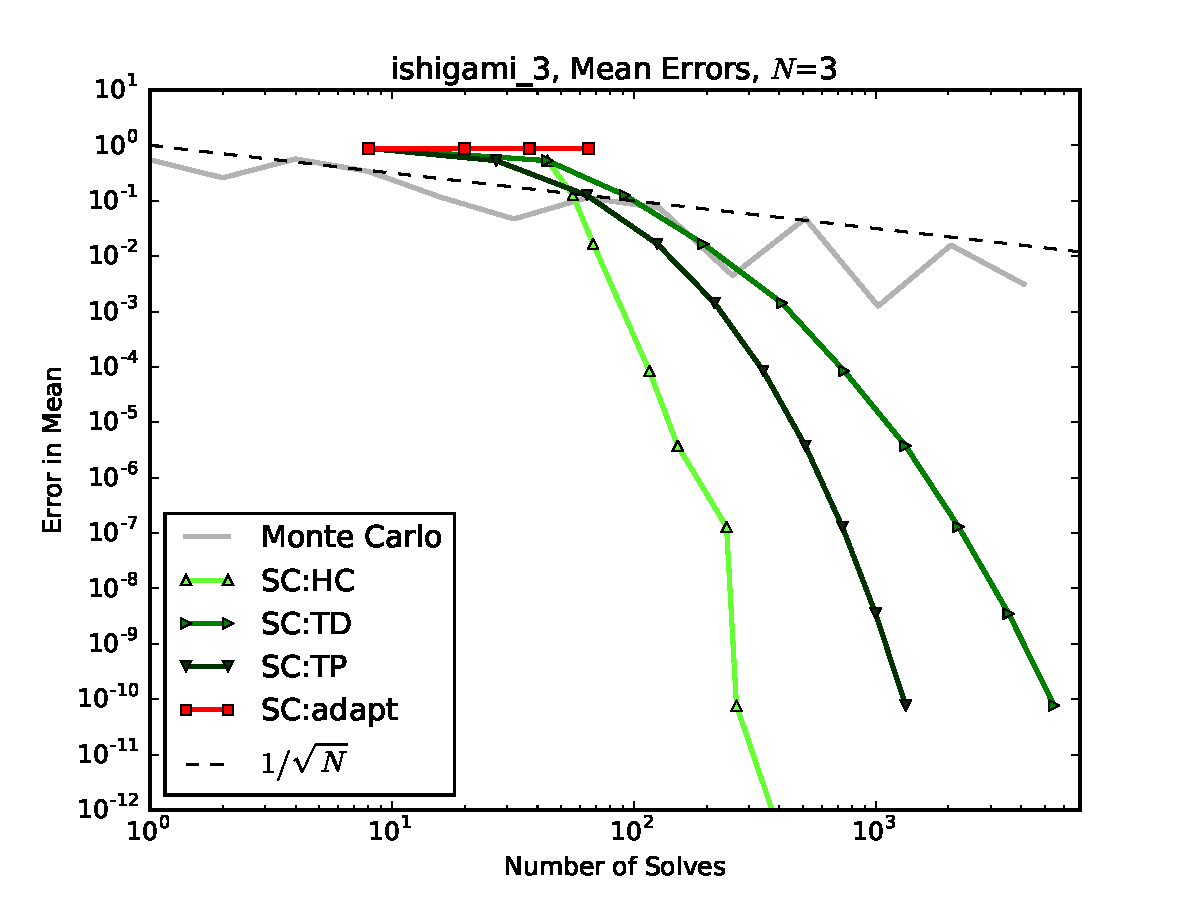
\includegraphics[width=0.7\linewidth]{anlmodels/ishigami_3_mean_errs_nohdmr}
  \caption{Ishigami, $N=3$, Mean Convergence}
  \label{fig:ishigami mean errors 3}
\end{figure}
\begin{figure}[H]
  \centering
  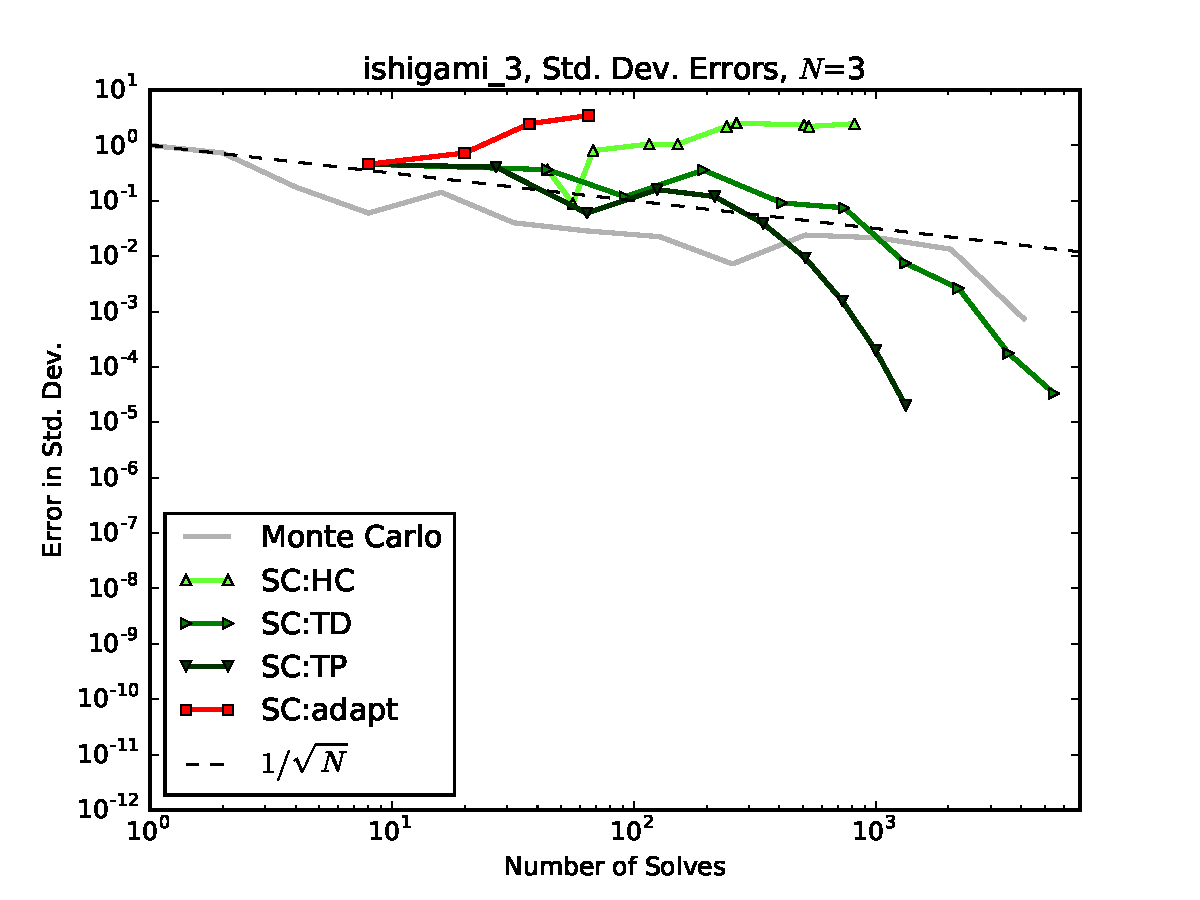
\includegraphics[width=0.7\linewidth]{anlmodels/ishigami_3_variance_errs_nohdmr}
  \caption{Ishigami, $N=3$, Std. Dev. Convergence}
  \label{fig:ishigami var errors 3}
\end{figure}


\section{Sobol G-Function}
\subsection{Description}
The so-called ``g-function'' introduced by Saltelli and Sobol \cite{gfunc} is a discontinuous
function used most commonly as a test for sensitivity coefficients.  The function is often used as an integrand
for numerical estimation methods \cite{gfuncM}.
The function is given by
\begin{equation}
  u(Y) = \prod_{n=1}^N \frac{\abs{4y_n-2}-a_n}{1+a_n},
\end{equation}
where
\begin{equation}
  a_n = \frac{n-2}{2}.
\end{equation}
The two-dimensional representation of this function is given in Figure \ref{fig: g func}.
\begin{figure}[htb]
  \centering
  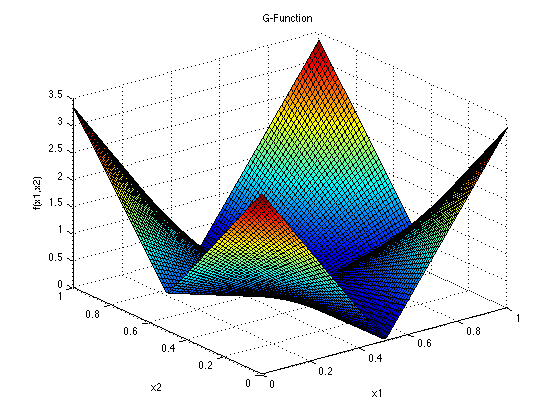
\includegraphics[width=0.7\linewidth]{anlmodels/gfunc}
  \caption{Sobol G-Function \cite{sfu}}
  \label{fig: g func}
\end{figure}

There are some implementations \cite{gfuncM} that force $a_n \geq 0$, which allows for a simple
understanding of the sensitivity coefficients:
\begin{itemize}
  \item $a_n=0$: $y_n$ is very important
  \item $a_n=1$: $y_n$ is relatively important,
  \item $a_n=9$: $y_n$ is non-important,
  \item $a_n=99$: $y_n$ is non-significant.
\end{itemize}
However, for our purposes, we set no limit to the value of $a_n$, as our interest is primarily in the moments
instead of the sensitivity coefficients.

We select this model because it offers the challenge of a function
without a continuous first derivative.  We expect the polynomial representations to perform poorly
in this instance, and more so as dimensionality increases.

\subsection{Discussion}
As expected, even for 3 input variables this discontinuous model provides a difficult challenges for
polynomial representations.  Even at thousands of computation solves, there is no discernible benefit in using
collocation methods over traditional Monte Carlo.  As with the Gaussian peak, the adaptive method completely
stalls in trying to converge this model.
\subsection{3 Inputs}
As evidenced in the figures, there is little justification for using any of the collocation methods for
uncertainty quantification with this model.  The level of discontinuity renders the benefits of the polynomial
expansions moot.
\begin{figure}[H]
  \centering
  \includegraphics[width=0.7\linewidth]{anlmodels/sobolG_3_mean_vals_nohdmr}
  \caption{Sobol G-Function, $N=3$, Mean Values}
  \label{fig:sobolG mean values 3}
\end{figure}
\begin{figure}[H]
  \centering
  \includegraphics[width=0.7\linewidth]{anlmodels/sobolG_3_var_vals_nohdmr}
  \caption{Sobol G-Function, $N=3$, Std. Dev. Values}
  \label{fig:sobolG var values 3}
\end{figure}

\begin{figure}[H]
  \centering
  \includegraphics[width=0.7\linewidth]{anlmodels/sobolG_3_mean_errs_nohdmr}
  \caption{Sobol G-Function, $N=3$, Mean Convergence}
  \label{fig:sobolG mean errors 3}
\end{figure}
\begin{figure}[H]
  \centering
  \includegraphics[width=0.7\linewidth]{anlmodels/sobolG_3_variance_errs_nohdmr}
  \caption{Sobol G-Function, $N=3$, Std. Dev. Convergence}
  \label{fig:sobolG var errors 3}
\end{figure}

\subsection{5 Inputs}
As with the smaller input space, it is clear that discontinuous models such as this are poor candidates for
collocation-based uncertainty analysis.
\begin{figure}[H]
  \centering
  \includegraphics[width=0.7\linewidth]{anlmodels/sobolG_5_mean_vals_nohdmr}
  \caption{Sobol G-Function, $N=5$, Mean Values}
  \label{fig:sobolG mean values 5}
\end{figure}
\begin{figure}[H]
  \centering
  \includegraphics[width=0.7\linewidth]{anlmodels/sobolG_5_var_vals_nohdmr}
  \caption{Sobol G-Function, $N=5$, Std. Dev. Values}
  \label{fig:sobolG var values 5}
\end{figure}

\begin{figure}[H]
  \centering
  \includegraphics[width=0.7\linewidth]{anlmodels/sobolG_5_mean_errs_nohdmr}
  \caption{Sobol G-Function, $N=5$, Mean Convergence}
  \label{fig:sobolG mean errors 5}
\end{figure}
\begin{figure}[H]
  \centering
  \includegraphics[width=0.7\linewidth]{anlmodels/sobolG_5_variance_errs_nohdmr}
  \caption{Sobol G-Function, $N=5$, Std. Dev. Convergence}
  \label{fig:sobolG var errors 5}
\end{figure}




\section{Conclusions}
todo
